\documentclass[12pt,a4paper]{report}

\usepackage{styles/dolgozat}

\usepackage{listings}
\usepackage{styles/cpp}
\usepackage{styles/python}
\usepackage{mathtools}
\usepackage{comment}

\usepackage{hyperref}

\begin{document}

\pagestyle{empty} %a címlapon ne legyen semmi=empty, azaz nincs fejléc és lábléc

% A Miskolci Egyetem címere
{\large
\begin{center}
\vglue 1truecm
\textbf{\huge\textsc{Szakdolgozat}}\\
\vglue 1truecm

\includegraphics[width=4.8truecm, height=4truecm]{images/me_logo.png}\\
\textbf{\textsc{Miskolci Egyetem}}
\end{center}}

\vglue 1.5truecm %függõleges helykihagyás

% A szakdolgozat címe, akár több sorban is
{\LARGE
\begin{center}
\textbf{Négykerekű járművek navigációs problémáinak megoldása}
\end{center}}

\vspace*{2.5truecm}
% A hallgató neve, évfolyam, szak(ok), a konzulens(ek) neve
{\large
\begin{center}
\begin{tabular}{c}
\textbf{Készítette:}\\
Tóth Péter\\
Mérnökinformatikus
\end{tabular}
\end{center}
\begin{center}
\begin{tabular}{c}
\textbf{Témavezető:}\\
Piller Imre
\end{tabular}
\end{center}}
\vfill
% Keltezés: Hely, év
{\large
\begin{center}
\textbf{\textsc{Miskolc, 2020}}
\end{center}}

\newpage


\newpage
\pagestyle{empty}

%Feladatkiiras
\begin{flushleft}
\textsc{\bfseries Miskolci Egyetem}\\
Gépészmérnöki és Informatikai Kar\\
Alkalmazott Matematikai Intézeti Tanszék\hspace*{4cm}\hfil \textbf{Szám:}
\end{flushleft}
\vskip 0.5cm
\begin{center}
\large\textsc{\bfseries Szakdolgozat Feladat}
\end{center}
\vskip 0.5cm
Tóth Péter (E445EX) mérnökinformatikus jelölt részére.\newline

\noindent\textbf{A szakdolgozat tárgyköre:} optimalizáció, navigáció, szimuláció, járművek\newline

\noindent\textbf{A szakdolgozat címe:} Négykerekű járművek navigációs problémáinak megoldása\newline

\noindent\textbf{A feladat részletezése:}

\medskip

\emph{Négykerekű járművek navigálási problémáinak részletes leírása. Feltételezzük, hogy a térkép felülnézetből ismert. Az optimalizálás célja azon navigációs műveleteknek a meghatározása, amely segítségével a jármű adott pozícióból a térkép járható területein keresztül el tud jutni a célként megadott pozícióba. Fel kell írni az optimalizálási feladatokat különböző célfüggvények figyelembevételével. Meg kell jeleníteni az algoritmus által adott útvonalakat. Az optimalizálási probléma megoldása Python programozási nyelven történik a NumPy függvénykönyvtár felhasználásával.}

\vfill

\noindent\textbf{Témavezető:} Piller Imre (egyetemi tanársegéd) \newline

% \noindent\textbf{Konzulens(ek):} (akkor kötelezõ, ha a témavezetõ nem valamelyik matematikai tanszékrõl való; de persze lehet egyébként is)\newline

\noindent\textbf{A feladat kiadásának ideje:}\newline

%\noindent\textbf{A feladat beadásának határideje:}

\vskip 2cm

\hbox to \hsize{\hfil{\hbox to 6cm {\dotfill}\hbox to 1cm{}}}

\hbox to \hsize{\hfil\hbox to 3cm {szakfelelős}\hbox to 2cm{}}

\newpage

\vspace*{1cm}  
\begin{center}
\large\textsc{\bfseries Eredetiségi Nyilatkozat}
\end{center}
\vspace*{2cm}  

Alulírott \textbf{Tóth Péter}; Neptun-kód: \texttt{E445EX} a Miskolci Egyetem Gépészmérnöki és Informatikai Karának végzős Mérnökinformatikus szakos hallgatója ezennel büntetőjogi és fegyelmi felelősségem tudatában nyilatkozom és aláírásommal igazolom, hogy \textit{Négykerekű járművek navigációs problémáinak megoldása}
című szakdolgozatom saját, önálló munkám; az abban hivatkozott szakirodalom
felhasználása a forráskezelés szabályai szerint történt.\\

Tudomásul veszem, hogy szakdolgozat esetén plágiumnak számít:
\begin{itemize}
\item szószerinti idézet közlése idézőjel és hivatkozás megjelölése nélkül;
\item tartalmi idézet hivatkozás megjelölése nélkül;
\item más publikált gondolatainak saját gondolatként való feltüntetése.
\end{itemize}

Alulírott kijelentem, hogy a plágium fogalmát megismertem, és tudomásul veszem, hogy
plágium esetén szakdolgozatom visszautasításra kerül.

\vspace*{3cm}

\noindent Miskolc, \hbox to 2cm{\dotfill} .év \hbox to 2cm{\dotfill} .hó \hbox to 2cm{\dotfill} .nap

\vspace*{3cm}

\hspace*{8cm}\begin{tabular}{c}
\hbox to 6cm{\dotfill}\\
Hallgató
\end{tabular}



\newpage

\noindent 1.

\begin{tabular}{cl}
&szükséges (módosítás külön lapon) \\
A szakdolgozat feladat módosítása& \\
& nem szükséges\\
&\\
\hbox to 4cm{\dotfill}&\multicolumn{1}{c}{\hbox to 5cm{\dotfill}}\\
dátum& \multicolumn{1}{c}{témavezető(k)}
\end{tabular}
\vskip1.5mm

\noindent 2. A feladat kidolgozását ellenőriztem:

\vskip1.5mm

\begin{tabular}{l@{\hspace*{4cm}}l}
témavezető (dátum, aláírás):& konzulens (dátum, aláírás):\\
\dotfill&\dotfill\\
\dotfill&\dotfill\\
\dotfill&\dotfill
\end{tabular}

\vskip1.5mm

\noindent 3. A szakdolgozat beadható:

\vskip1.5mm

\begin{tabular}{@{\hspace*{1.3cm}}c@{\hspace*{2.1cm}}c}
\hbox to 4cm{\dotfill}&\multicolumn{1}{c}{\hbox to 5cm{\dotfill}}\\
dátum& \multicolumn{1}{c}{témavezető(k)}
\end{tabular}

\vskip1.5mm

\noindent 4.
\begin{tabular}[t]{@{}l@{\hspace*{1mm}}l@{\hspace*{1mm}}l@{}}
A szakdolgozat& \hbox to 3.5cm{\dotfill} &szövegoldalt\\
              & \hbox to 3.5cm{\dotfill} &program protokollt (listát, felhasználói leírást)\\
              &\hbox to 3.5cm{\dotfill}   &elektronikus adathordozót (részletezve)\\
              &\hbox to 3.5cm{\dotfill} & \\
              &\hbox to 3.5cm{\dotfill} &egyéb mellékletet (részletezve)\\
              &\hbox to 3.5cm{\dotfill} &\\
\end{tabular}
\newline tartalmaz.

\vskip1.5mm

\begin{tabular}{@{\hspace*{1.3cm}}c@{\hspace*{2.1cm}}c}
\hbox to 4cm{\dotfill}&\multicolumn{1}{c}{\hbox to 5cm{\dotfill}}\\
dátum& \multicolumn{1}{c}{témavezető(k)}
\end{tabular}

\noindent 5.

\begin{tabular}{ll}
&bocsátható\\
A szakdolgozat bírálatra& \\
& nem bocsátható\\
\end{tabular}

\vskip1.5mm

\noindent A bíráló neve: \hbox to 8cm{\dotfill}

\vskip4mm

\begin{tabular}{@{\hspace*{1.3cm}}c@{\hspace*{2.1cm}}c}
\hbox to 4cm{\dotfill}&\multicolumn{1}{c}{\hbox to 5cm{\dotfill}}\\
dátum& \multicolumn{1}{c}{szakfelelős}
\end{tabular}

\noindent 6.
\begin{tabular}[t]{@{}l@{\hspace*{1mm}}l@{\hspace*{1mm}}l@{}}
A szakdolgozat osztályzata& &\\
&a témavezető javaslata:& \hbox to 3cm{\dotfill}\\
&a bíráló javaslata:& \hbox to 3cm{\dotfill}\\
&a szakdolgozat végleges eredménye:& \hbox to 3cm{\dotfill}
\end{tabular}

\vspace*{4mm}

\noindent Miskolc, \hbox to 4.5cm{\dotfill} \hspace*{2.5cm}
\begin{tabular}[t]{cc}
\hbox to 6cm{\dotfill}\\
a Záróvizsga Bizottság Elnöke
\end{tabular}


\cleardoublepage
\pagenumbering{gobble}
\tableofcontents
\cleardoublepage
\pagenumbering{arabic}

\newpage

\pagestyle{fancy}

\Chapter{Bevezetés}

A négykerekű járművek mozgása sokféle tudományág definícióiból határozható meg a való életben. A dolgozatomban alapvetően a járművet geometriai és kinematikai szemszögből vizsgálom meg, az ezen tudományágak definíciói segítségével szeretnék néhány problémára kitérni, amik szóba jöhetnek navigációs szempontból.

Az egyik alapvető probléma például, hogy egy jármű egyik pontból a másikba kellene, hogy eljusson. Ezt különböző algoritmusok segítségével tudjuk kivitelezni, amely valamilyen logika alapján meghatároz egy útvonalat végeredményként. Kezdésként a véletlen számok használatával juttatnám el a járművet bizonyos pontokba, és megláthatjuk, milyen paraméterek alapján mely pozíciókba juthatunk el a legnagyobb valószínűséggel. Mivel ez az eredmény még nem tekinthető optimálisnak, szükség lesz egy keresőalgoritmusra, ami eleget tesz bizonyos alapkövetelményeknek. Ez esetben az egyik fontosabb célfüggvény a legrövidebb útvonalat jelentené a két pont között.

A következő esetben egy jármű mozgását szeretném szimulálni egy parkolóban. Itt meg kell határoznunk, hogy melyik parkolóhelyről, melyik másikba álljon át az autó, valamint orral vagy háttal. Ehhez meg kell oldani, hogy a kiszámított útvonalat tudja követni a jármű. Itt a különböző irányvektorok, valamint a szögek váltakozása fog érdekes problémát adni.

Mindenféle mozgás vagy útvonal tervezés a dolgozatomban kétdimenziós környezetben történik. A Descartes-féle koordinátarendszert veszem alapul a pozícionálásokhoz és az egyéb pontok meghatározásához. Így is fogom az eredményeket ábrázolni, melyek képként lesznek megjelenítve minden eset után, valamint ezeken az $ x $ és $ y $ koordináták be lesznek skálázva, így szemléltetem a pozíciót.

Végeredményként szeretnék majd a parkolós mozgásról kezdetleges animációkat bemutatni, hogy hogyan képes az adott paraméterek alapján az autó navigálni és célba érkezni. Ezeket .gif kiterjesztésű mozgókép formában szemléltetném majd, amelyek a dolgozat mappájában elérhetőek lesznek.

Minden ilyen teszt esetet python nyelven implementáltam, ezen kódrészeket is be fogom mutatni és rögtön utána egy-egy példát is, mint futtatási eredményt kép formájában. Kitérek azokra a matematikai definíciókra is, amik alapján a kód készült. Ezeket részletesen le fogom vezetni és ábrákkal is szemléltetem a későbbiekben a definiált változókat.



\Chapter{A járművek mozgásának modellezése}

\Section{Kétkerekű modell kanyarodási íve}

Érdemes lehet előrször a kétkerekű modellt megvizsgálnunk, ugyanis az itt meghatározott képletek adják alapul a négykerekű változatnál használt formulákat. Először is meg kell határoznunk a kanyarodás ívét, ami jelen esetben egy adott elfordulási ($\alpha$) szög mellett tehető meg. Ahogy ez a szög változik úgy fog változni maga az ív is, amin a jármű haladni fog. Ezért első lépésben a sugarat kell megkeresnünk, mert az adott sugárral a középpont köré húzható kör fogja adni az útvonalat. 
A kétkerekű (bicikli) modell kanyarodási ívének meghatározása 2 dologtól függ:\newline
\phantom{len} - a tengelytávolságtól (w),\newline
\phantom{len} - az első kerék kanyarodási szögétől ($\alpha$).\newline
Az első és hátsó kerekek is egy-egy körpályát fognak követni azonos középponttal. Az irány mindig merőleges a sugárra.

\begin{figure}[h!]
\centering
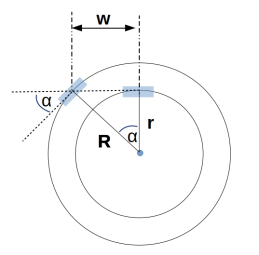
\includegraphics[scale=0.5]{images/two_wheels_rad.png}
\caption{Kétkerekű jármű kanyarodási íve}
\label{fig:two_wheels_rad}
\end{figure}
A \ref{fig:two_wheels_rad} ábrán R az első kerékhez tartozó sugár, r pedig a hátsó kerékhez.\\
Az első kerék pályája: $\sin\alpha$ = $\cfrac{w}{R}$ \hspace{5mm}---> \hspace{5mm} $R$ = $\cfrac{w}{\sin\alpha}$ \\
A hátsó kerék pályája: $\tan\alpha$ = $\cfrac{w}{r}$ \hspace{5mm}---> \hspace{5mm} $r$ = $\cfrac{w}{\tan\alpha}$
\\

Itt a szögfüggvényekben való eltérést a \ref{fig:two_wheels_rad} ábrán látható háromszögől leolvashatjuk, miszerint első kerék esetén a derékszögű háromszög átfogója lesz a sugár, így a kanyarodási szög szinuszát vesszük, a hátsó kerék esetén pedig a szög melletti befogó lesz a sugár, tehát a tangensét kell néznünk. Így átalakítva a képletet megkapjuk a két sugarat.   


\Section{A jármű matematikai modellje}

Áttérve a négykerekű járművekre szintén meg lehet határozni mind a négy kerékhez tartozó sugarat. A \ref{fig:each_wheel_radius}. ábra egy kicsivel részletesebb modellt szemléltet, amin megjelölöm mind a négy sugarat. Az ábrán az úgynevezett Ackerman kanyarodási geometria lényege is látható egy nagyon egyszerű szemléltetéssel, ami megoldja az első két kerék különböző szögekbe való fordítását, ha a jármű fizikai felépítését vesszük. A sugarak kiszámításához képletek a következők:
\\
$R_{IF}$ =  $\cfrac{w}{\sin\alpha_1}$ - $\cfrac{a}{2}$\qquad
$R_{IR}$ =  $\cfrac{w}{\tan\alpha_1}$ - $\cfrac{a}{2}$\\
$R_{OF}$ =  $\cfrac{w}{\sin\alpha_2}$ + $\cfrac{a}{2}$\qquad
$R_{OR}$ =  $\cfrac{w}{\sin\alpha_1}$ + $\cfrac{a}{2}$\\

\begin{figure}[h!]
\centering
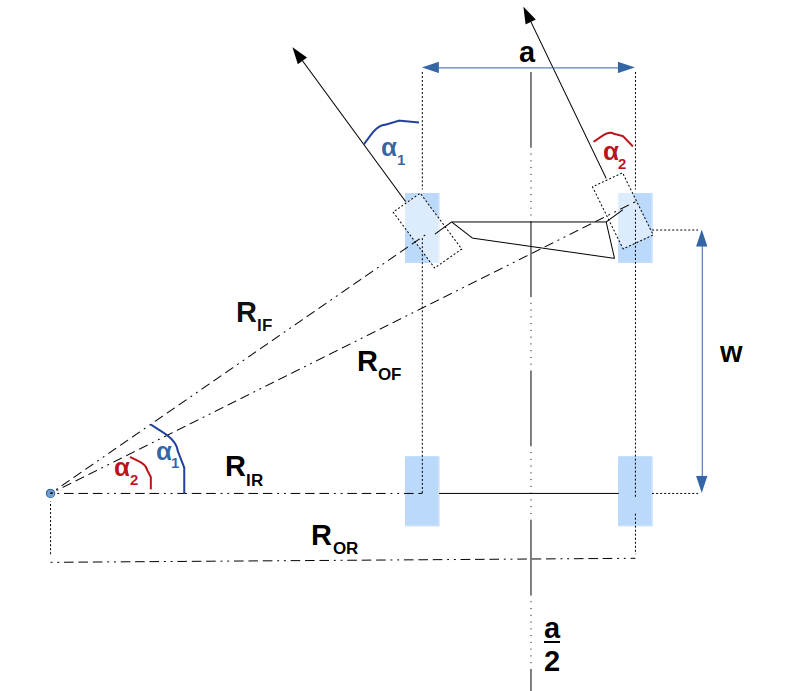
\includegraphics[scale=0.45]{images/each_wheel_radius.png}
\caption{Jármű kerekeinek sugarai}
\label{fig:each_wheel_radius}
\end{figure}

Itt az első kerekeknél a sugár az átfogót képezné, míg a hátsó kerekeknél a szög melletti befogót. Ezért is váltakozik a szinusz és a tangens a trigonometriai összefüggések hatására. Az $\cfrac{a}{2}$ pedig attól függően, hogy a kanyarodás irányához viszonyítva a külső vagy belső kerekekről van szó, a tengely hosszának a felét elvesszük vagy hozzáadjuk a képlethez. 

\subsection{Korábbi technológiák:}

Szeretném egy kicsit részletesebben (kezdetitől a modernebb megoldásokig) bemutatni a jármű modelljét és a kanyarodási elveket/technológiákat. 

A kanyarodás az első kerekek elforgatásával történik. Az első ilyen koncepciónál magát a tengelyt lehetett kormányozni, nem pedig a kerekeket. Ez a megoldás a lassú haladáshoz és a könnyebb manőverezéshez előnyös lehet, de az első tengelynek nagy ívben el kell fordulnia a kanyarodástól függően valamelyik irányba. Ez a futómű kialakítását nagy mértékben korlátozza, maga a felfüggesztés megoldása is nagy kihívás lehet ezt a technológiát alkalmazva.

A kanyarodás következő megoldásánál már mindkét első kerék külön-külön forgatható, de azonos az elfordulási szög. Ebben az esetben a jármű dinamikáját nézve úgynevezett oldal irányú csúszás tapasztalható a kerekeken (a kanyarodás irányának függvényében). Ebben közrejátszik, hogy mivel mindkét kerék egy irányba néz ha el van fordítva a kormány, 2 különböző középpontja lesz a forgásnak, így legalább az egyik kerék csúszni fog a kanyarodáskor.

Ideális megoldásnak vesszük azt az esetet, mikor mindkét első kereket egymástól függetlenül lehet kormányozni. Ebben az esetben mindkét kerék kanyarodási szögét meg lehetne úgy határozni, hogy a kerék középpontja egy érintő egyenes lenne a közös kanyarodási középpontból húzható körívre. Így megválasztva a megfelelő sugarat a körívnek, mindkét kereket tekintve elkerülhető az oldal irányú csúszás. A fejezet további ehhez kapcsolódó pontjai is ezt a megoldást fogják tovább részletezni.\\

Definiálnunk kell különböző jelöléseket, melyek segítségével a képletek leírhatók és értelmezhetők. A négykerekű jármű középpontjának a hátsó tengely középpontját tekintjük. Vagyis esetünkben az elforduláshoz szükséges számításoknál ezt vesszük figyelembe. Mivel a kanyarodásnál az első kerekek különböző szögeket zárnak be az első tengellyel, ezért érdemes egy képzeletbeli, az első tengely közepére eső kormányozható kereket megadni. Ennek a jármű irányával bezárt előjeles szögét jelöljük $\alpha$-val. A jármű tengelytávolságát jelöljük $w$-vel, a hátsó tengely hosszát pedig $a$-val (\ref{fig:vehicle}. ábra).

\begin{figure}[h!]
\centering
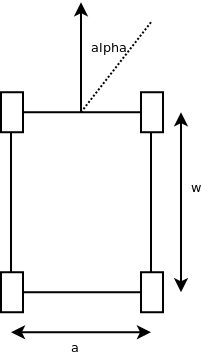
\includegraphics[scale=0.45]{images/vehicle.png}
\caption{A jármű matematikai modelljének fő paraméterei}
\label{fig:vehicle}
\end{figure}

\Section{Első kerekek elfordulási szögének kiszámítása}

A kanyarodásnál tehát figyelembe kell venni, hogy a két első kerék különböző szögben fordul el, mégpedig az iránytól függően a belső kerék nagyobb szögben tér el az egyenestől, míg a külső kisebb szögben. Minél nagyobb a kanyarodási szög, annál nagyobb az eltérés a két kerék elfordulásában.
Az $\alpha$ szög függvényében külön ki kell számítanunk a jármű bal és jobb első kerekének elfordulási szögét.
Tehát első lépésben határozzuk meg az adott $\alpha$ szög ismeretében a további számításokhoz szükséges sugarat,
melyet a \ref{fig:turning_vehicle}. ábrán R jelöl. Ez a kanyarodási sugár, melyet a jármű középvonalához mérünk.
Az ehhez szükséges képlet:\vspace{2mm}
$R$ = $\dfrac{w}{\text{tg} \alpha}$ \vspace{5mm}

Továbbiakban a jelölések ugyanazok, az első kerekeket tekintve pedig $\alpha_1$ a belső, $\alpha_2$ pedig a külső kerék elfordulási szögét jelöli.  
A jármű tengelytávolsága, valamint szélessége, és a sugár ismeretében ezen két szög a következőképpen számítható ki:\vspace{5mm}

$\alpha\textsubscript{1}$ = $\text{arctan}\Bigg(\cfrac{w}{R-\frac{a}{2}}\Bigg)$ \hspace{1cm} $\alpha\textsubscript{2}$ = $\text{arctan}\Bigg(\cfrac{w}{R+\frac{a}{2}}\Bigg)$\vspace{5mm}

\begin{figure}[h!]
\centering
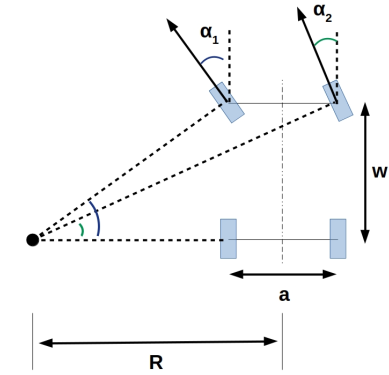
\includegraphics[scale=0.5]{images/turning_vehicle.png}
\caption{Első kerekek elfordulási szögei}
\label{fig:turning_vehicle}
\end{figure}
\vspace{5mm}


A kanyarodási sugárból átalakítható a képlet a trigonometrikus összefüggéseket figyelembe véve. A szögeket megkaphatjuk, ha a képletet rendezzük úgy, hogy a tangens inverzével szorozva elosztjuk a tengelytávolságot az adott kerékhez tartozó sugárral. Ugyanis az arkusz tangens visszaadja azt a szöget, ami jelen esetben a sugárhoz és a tengelytávolsághoz tartozik. Mivel mindkét keréknek más lesz a sugara a kijelölt ponttól, ezeket is külön meg kell határozni, így a képlet nevezőjében a kanyarodási középponthoz közelebb eső kerékhez tartozó sugárból kivonjuk a jármű szélességének felét, míg a messzebb eső kerékhez hozzáadjuk ezt az értéket.

% TODO: Részletesen leírni ezek számítását!

\Section{Pozíció számítása rögzített $\alpha$ mellett}

A rögzített $\alpha$ szög, és adott sebesség mellett ki kell tudnunk számolni, hogy adott $(x_0, y_0)$ kiindulópontból indulva a jármű milyen pozícióba fog kerülni $t$ idő elteltével. Az $\alpha$ szög függvényében az alábbi módon számolhatjuk ki annak a képzeletbeli körnek a sugarát ($R$), amelyen a jármű majd kanyarodni fog:
\[
R = \dfrac{w}{\text{tg} \alpha},
\]
ahol a $w$ a jármű tengelyei közötti távolságot jelöli.

Tegyük fel, hogy a jármű sebessége $v$. Ekkor $t$ idő függvényében a jármű pozícióját az alábbi formában számolhatjuk:
\begin{align*}
x(t) &= x_0 + R - R \cdot \cos \dfrac{v \cdot t}{|R|}, \\
y(t) &= y_0 + |R| \cdot \sin \dfrac{v \cdot t}{|R|}.
\end{align*}

\Section{Útvonal meghatározása az eltelt idő függvényében}

$$
\vec{v} \in \mathbb{R} \hspace{0.5cm}
\quad \rightarrow \quad
\vec{v} (t) \colon \mathbb{R} \to \mathbb{R}^2
$$

Elfordulás:
$$
\varphi (t) \hspace{0.5cm} \rightarrow \hspace{0.5cm} \vec{v} (t) =
\begin{bmatrix}
\cos(\varphi(t)) \\
\sin(\varphi(t))
\end{bmatrix}
$$

$ \vec{x_0} $ : kezdőpozíció

Egy egységnyi idő elteltével az irány: $ \vec{x} (t_1) = \vec{x_0} + \displaystyle\int_{t_0}^{t_1} \vec{v} (t) dt $

Általános alak:  $ \vec{x} (t) = \vec{x_0} + \displaystyle\int_{t_0}^{t} \vec{v} (u) du $

$$
\begin{bmatrix} x_1 \\ y_1 \end{bmatrix} = \begin{bmatrix} x_0 \\ y_0 \end{bmatrix} + \displaystyle\int_{t_0}^{t_1} \begin{bmatrix} \cos(\varphi(t)) \\ \sin(\varphi(t)) \end{bmatrix} dt 
$$


Külön a két vektort leintegráljuk:
\begin{align*}
x_1 &= x_0 + \displaystyle\int_{t_0}^{t_1} \cos(\varphi(t)) \; \mathrm{d}t \\ \\
y_1 &= y_0 + \displaystyle\int_{t_0}^{t_1} \sin(\varphi(t)) \; \mathrm{d}t \\
\end{align*}

Az integrálás kifejtése:
\begin{align*}
x_1 = x_0 + \left[\dfrac{1}{\varphi} \cdot \sin(\varphi(t))\right]_{t_0}^{t_1} = x_0 + \left(\left(\dfrac{1}{\varphi} \cdot \sin(\varphi({t_1)})\right) - \left(\dfrac{1}{\varphi} \cdot \sin(\varphi({t_0}))\right)\right)  \\ \\
y_1 = y_0 + \left[- \dfrac{1}{\varphi} \cdot \cos(\varphi(t))\right]_{t_0}^{t_1} = y_0 + \left(\left(- \dfrac{1}{\varphi} \cdot \cos(\varphi({t_1)})\right) - \left(- \dfrac{1}{\varphi} \cdot \sin(\varphi({t_0}))\right)\right) \\
\end{align*}

Ezzel a számítással megkaphatjuk a jármű által bejárt utat. Jelen esetben a képlet mindig csak a következő pozítiót adja meg, tehát $x_1$ jelentené a következő pozíciót, $x_0$ az előzőt. Az idő szintén a nulladik és az első időpillanatra vonatkozik ($t_0$, $t_1$), valamint a kanyarodási szög mindig az aktuális. Ennek a szögnek az értékénél figyelembe kell venni, hogy negatív vagy pozitív szám. Ez megadja, hogy melyik irányba kanyarodik a jármű a 0 fokhoz képest (ami azt jelenti, hogy előre felé néz). Ha a $\varphi$ < 0 akkor jobbra, ha $\varphi$ > 0  akkor balra fog kanyarodni.

\Section{A jármű mozgása és pozícionálása}

Ebben a pontban szeretném bemutatni a jármű mozgása közben megoldandó pozícionálási problémát. Tehát egy autó-szerű objektumot fogunk vizsgálni, amint megpróbál eljutni egyik pontból a másikba, figyelembe véve azt is, hogy mi a kezdő és végpozíció irányvektora. Továbbra is egy kétdimenziós környezetben fogjuk nézni a jármű mozgását, valamint a kétkerekű modell alapján beállítani a paramétereit. A jármű középpontja a hátsó tengely közepe lesz, így a forgásközéppont a négykerekű járműre illesztett kétkerekű modell hátsó kerekének közepére fog esni. \\\\
Ebben az esetben alapvetően három paraméterrel tudjuk a jármű pozícióját reprezentálni:
\begin{itemize}
	\item x pozíció
	\item y pozíció
	\item $ \delta $ irányszög
\end{itemize}
A számításokhoz a sebességet is figyelembe kell majd venni, ami a jármű pozícióját tekintve x irányban kap értéket, y-ban pedig mindig 0 lesz, ezzel elkerülve az oldal irányú csúszást a kerekek mozgásának megfelelően. A \ref{fig:position} ábrán ezt a részt a szaggatott vonalakkal jelölöm, amik mindig merőlegesek a jármű kerekeire és a forgásközéppontból indulnak. A jármű referenciapontja mindig egy kör alakú pályát követ, aminek a szögsebessége a következő képlettel leírható:\\

$\dot{\delta} = \dfrac{v}{R},$ \\\\
ahol $ v $ a sebesség, $ R $ pedig a hátsó kerék körpályájának a sugara. A későbbiekben $ \gamma $-val jelöljük majd a kanyarodási szöget, ami egy bizonyos értéknél nem lehet nagyobb, tekintve a jármű mechanikáját. Ennek a szögnek a maximum értéke határozza meg a kanyarodási ív sugarának minimális értékét. Egy állandó kanyarodási szög mellett az autó egy körpályán halad, ami miatt a bejárni kívánt út ilyen körívekből épül fel. Tehát minden időpillanatban a kanyarodási szög kis mértékben változik, így az út követése egyszerűbbé válik. Ha egy négykerekű járművet veszünk figyelembe, akkor a kormányzott kerekek különböző sugarú íveket járnak be, és ezzel együtt a két kanyarodó kerék különböző szögekben is fordulnak el. Tehát itt $ \gamma_{inner} $  és $ \gamma_{outer} $ szögeket is meg kell különböztetni, mint a kanyarodás irányát tekintve külső és belső elfordulási szögeket az Ackerman mechanizmus alapján. 
A jármű paraméterei a következő mozgási egyenlet szerint fognak változni:
\begin{itemize}
	\item[] $ \dot{x} = v \cdot \cos\delta $
	\item[] $ \dot{y} = v \cdot \sin\delta $
	\item[] $ \dot{\delta} = \dfrac{v}{L} \cdot \tan\gamma $
\end{itemize}

Melynek $ \dot{\delta} $ értéke a $ \dot{\delta} = \dfrac{v}{R} $ képletből adódik. Ennek geometriai részletezése a metametikai modell résznél található a koncepció fejezetben. 

Ezen modell a kinematikai modellnek felel meg, miszerint a jármű mozgását definiáljuk és nem a járműre ható erőket és egyéb környezeti hatásokat. Maga a pozíció változását a $ \delta $ fogja jelölni ( vagy $ \dot{\delta} $ ), melynek értékét az imént felvezetett irányszög képlete adja. A leírtakat a \ref{fig:position} ábrán keresztül szemléltetem.\\

\begin{figure}[h!]
\centering
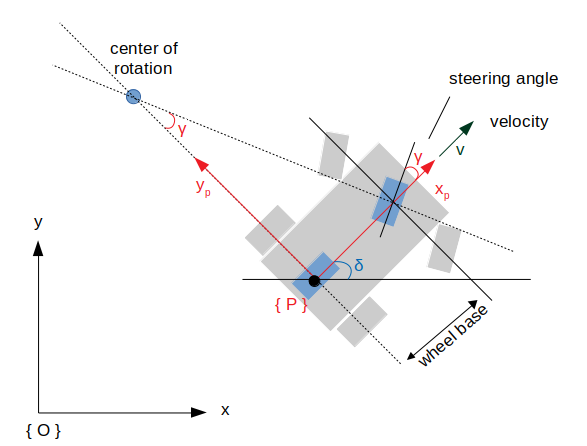
\includegraphics[scale=0.70]{images/position.png}
\caption{A jármű mozgása}
\label{fig:position}
\end{figure}

Az imént felvezetett egyenlet egyéb fontosabb karakterisztikákat is realizál, miszerint $ v = 0-ban$ $ \delta = 0 $, ami azt jelenti, hogy nem tudjuk a jármű orientációját változtatni, ha az nincs mozgásban. Másként: a járműnek muszáj haladnia annak érdekében, hogy fordulni tudjunk vele. 

Ahhoz, hogy el tudjunk mozdulni egy adott pontba, a sebességet arányosan kell változtatni a célhoz való távolság függvényében. Ekkor a következő képletet alkalmazhatjuk:\\

$ v = K \cdot \sqrt{(x\_goal - x)^2 + (y\_goal - y) ^2}$ \\

Valamint a kormányzást a célpozíció felé (ami esetünkben a jármű relatív kanyarodási szögét jelenti) a következő képpen tudjuk definiálni:\\

$ \delta\_goal = \tan^{-1} \cdot \dfrac{y\_goal - y}{x\_goal - x} $\\

valamint a kanyarodási szöget be kell állítani úgy, hogy az a végpontbeli állapot felé irányuljon:\\

$ \gamma = K \cdot ( \delta\_goal \cdot \delta ) $, \qquad ahol $ K > 0 $\\

Így eljutottunk a problémához, hogy a járművet egy bizonyos pozícióba kell irányítani $ (x\_goal, y\_goal, \delta\_goal) $. Az előbbiekben meghatározott képletek segítségével eljuthatunk ebbe a pozícióba a kezdőpozíció ismeretének függvényében. Először is a mozgási egyenletet át kell írnunk mátrix formába, ami a következő képpen fog alakulni:\\

\( \begin{pmatrix}
	\dot{x}\\
	\dot{y}\\
	\dot{\delta}
\end{pmatrix} \)
=
\( \begin{pmatrix}
	\cos\delta & 0\\
	\sin\delta & 0\\
	0 & 1
\end{pmatrix} \)
$ \cdot $ 
\( \begin{pmatrix}
	v\\
	\gamma
\end{pmatrix} \)
\\\\\\
Ezek alapján a ezeket változókat vezethetjük be, hogy irányítani tudjuk a járművet a célban megadott pozíció felé:
\begin{itemize}
	\item[] $ dist = \sqrt{\Delta x^2 + \Delta y^2} $
	\item[] $ \alpha = \tan^{-1} \cdot \dfrac{\Delta y}{\Delta x} - \delta $
	\item[] $ \beta = -\delta - \alpha $
\end{itemize}
 
Ezeket szintén mátrix formába rendezve a következőket kapjuk:\\

\( \begin{pmatrix}
	\dot{dist}\\
	\dot{\alpha}\\
	\dot{\beta}
\end{pmatrix} \)
=
\( \begin{pmatrix}
	\cos\alpha & 0\\\\
	\dfrac{\sin\alpha}{dist} & -1\\\\
	-\dfrac{\sin\alpha}{dist} & 0
\end{pmatrix} \)
$ \cdot $ 
\( \begin{pmatrix}
	v\\
	\gamma
\end{pmatrix} \)
\\\\\\
és feltételezve, hogy a célpozíció a jármű előtt van, az autó irányítása így történik:\\

$ v = K_{dist} \cdot dist $\\

$ \gamma = K_\alpha \cdot \alpha + K_\beta \cdot \beta $\\\\
ahol a konstans értékekre a következő feltételek vonatkoznak: $ K_{dist} > 0, \quad K_\beta < 0, \quad K_\alpha - K_\beta > 0  $\\
Ellenkező esetben ennek az alkalmazott sebességnek a negáltját kell vennünk, tehát tolatni kell a járművel:\\

$ v = -v $, \qquad ha $\alpha \not\in \left(-\dfrac{\pi}{2}, \dfrac{\pi}{2} \right) \quad $ (ez cél szerint változtatható lesz)\\\\
Az lenne a lényege ennek a megoldásnak, hogy a a definiált képletek $ K_{dist} \cdot dist $ és $ K_\alpha \cdot \alpha $ egy vonal mentén vezetik a járművet a cél felé, amíg $ K_\beta \cdot \beta $ ezt a vonalat folyamatosan a cél irányba fordítja.

\begin{figure}[h!]
\centering
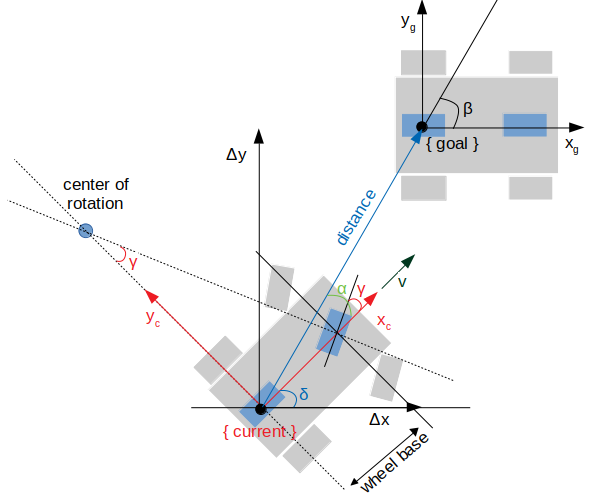
\includegraphics[scale=0.70]{images/moving_vehicle.png}
\caption{A jármű mozgása}
\label{fig:moving_vehicle}
\end{figure}

\subsection{Rotációs mátrix definiálása}

A pozícionáláshoz szükséges pontokat, vektorokat és az azokkal végzett műveleteket szeretném egy kicsit részletezni. Mint már említettem, itt is egy Descartes-féle koordinátarendszerben dolgozunk, melyben egy-egy ponthoz az $ x $ és $ y $ tengely irányába mutató egységvektorok is tartoznak, tehát egy pont így írható le:\\

$ P = x\vec{x} + y\vec{y} $\\\\
Az A-ból B-be való eljutás egyfajta eltolás lesz az A koordinátán. Vagy inkább koordinátarendszeren, mivel a forgatást tekintve a tengelyek, mint vektorok is más-más irányba mutatnak majd. Tehát mondjuk, hogy a B koordináta el lett tolva egy $ t = (x, y) $ vektor által és el lett forgatva egy $ \delta $ szöggel. Ezt a \ref{fig:a_to_b_point} ábra szemlélteti:

\begin{figure}[h!]
\centering
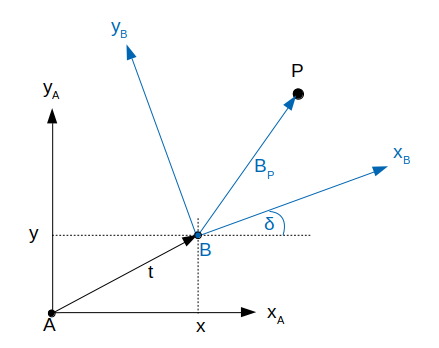
\includegraphics[scale=0.70]{images/A_to_B_point.png}
\caption{A jármű mozgása}
\label{fig:a_to_b_point}
\end{figure}

\newpage

Ha csak a helyzet változást vesszük figyelembe, akkor egy olyan elmozdulást tapasztalunk, amikor a kapott pont tengelyei párhuzamosak a kezdőpontéra. Legyen ez az új pont $ T $, és az imént felírt képlet alapján:\\

$ {}^{T}p = {}^{T}x\vec{x}{}_{T} + {}^{T}y\vec{y}{}_{T} $  =
\(
\begin{pmatrix}
	\vec{x}{}_{T} & \vec{y}{}_{T}
\end{pmatrix}	 
\)
\(
\begin{pmatrix}
	{}^{T}x\\
	{}^{T}y
\end{pmatrix}	 
\)\\\\
A $ B $ pont, már az elforgatást is tartalmazza, mely 2 egység vektorral írható le:\\

$ \vec{x}{}_{B} = \cos\delta\vec{x}{}_{T} + \sin\delta\vec{y}{}_{T} $\\

$ \vec{y}{}_{B} = -\sin\delta\vec{x}{}_{T} + \cos\delta\vec{y}{}_{T} $\\\\
ami mátrix formában felírva a következő:\\

\(
\begin{pmatrix}
	\vec{x}{}_{B} & \vec{y}{}_{B}
\end{pmatrix}
\) =
\(
\begin{pmatrix}
	\vec{x}{}_{T} & \vec{y}{}_{T}
\end{pmatrix}
\)
\(
\begin{pmatrix}
	\cos\delta & -\sin\delta\\
	\sin\delta & \cos\delta
\end{pmatrix}
\)\\\\
A keresett $ P $ pont pedig az előzőekhez hasonlóan felírva:\\

$ {}^{B}p = {}^{B}x\vec{x}{}_{B} + {}^{B}y\vec{y}{}_{B} $  =
\(
\begin{pmatrix}
	\vec{x}{}_{B} & \vec{y}{}_{B}
\end{pmatrix}	 
\)
\(
\begin{pmatrix}
	{}^{B}x\\
	{}^{B}y
\end{pmatrix}	 
\)\\\\
Majd $ B $-vel megszorozva:\\

$ {}^{B}p $ =
\(
	\begin{pmatrix}
		\vec{x}{}_{T} & \vec{y}{}_{T}
	\end{pmatrix}
\)
\(
	\begin{pmatrix}
		\cos\delta & -\sin\delta\\
		\sin\delta & \cos\delta
	\end{pmatrix}
\)
\(
\begin{pmatrix}
	{}^{B}x\\
	{}^{B}y
\end{pmatrix}	 
\)\\\\
Majd a jobb oldali együtthatókat egyenletként felírva a következőt kapjuk:\\

\(
	\begin{pmatrix}
		\vec{x}{}_{T} & \vec{y}{}_{T}
	\end{pmatrix}
\) = 
\(
	\begin{pmatrix}
		\cos\delta & -\sin\delta\\
		\sin\delta & \cos\delta
	\end{pmatrix}
\)
\(
\begin{pmatrix}
	{}^{B}x\\
	{}^{B}y
\end{pmatrix}	 
\qquad \Rightarrow \qquad\)  
\(
	\begin{pmatrix}
		\vec{x}{}_{T} & \vec{y}{}_{T}
	\end{pmatrix}
\) = 
$ {}^{T}R{}_{B} $
\(
\begin{pmatrix}
	{}^{B}x\\
	{}^{B}y
\end{pmatrix}	 
\)\\\\

\begin{figure}[h!]
\centering
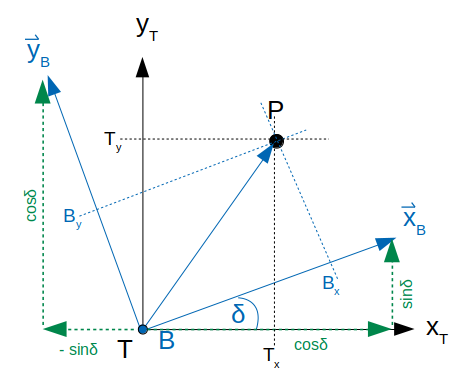
\includegraphics[scale=0.70]{images/T_to_B_point.png}
\caption{A jármű négy pontja a programban}
\label{fig:t_to_b_point}
\end{figure}

És ezzel leírtuk, hogyan forgattuk el a $ T $ pontot a $ B $ pontba. Ez lenne maga a rotációs mátrix. A fent leírt műveleteket a \ref{fig:t_to_b_point} ábra szemlélteti.
\\\\
Ehhez még hozzá kell adnunk az eltolást, ami az $ A $ pontból a $ B $ pontba történik. Ezt egy egyszerű vektoros hozzáadással tehetjük meg:\\


\(
\begin{pmatrix}
	{}^{A}x\\
	{}^{A}y
\end{pmatrix}	 
\) = 
\(
\begin{pmatrix}
	{}^{T}x\\
	{}^{T}y
\end{pmatrix}	 
\) + 
\(
\begin{pmatrix}
	x\\
	y
\end{pmatrix}
\) =
\(
\begin{pmatrix}
	\cos\delta & -\sin\delta\\
	\sin\delta & \cos\delta
\end{pmatrix}
\)
\(
\begin{pmatrix}
	{}^{B}x\\
	{}^{B}y
\end{pmatrix}	 
\) + 
\(
\begin{pmatrix}
	x\\
	y
\end{pmatrix}	 
\)\\\\ = 
\(
	\begin{pmatrix}
		\cos\delta & -\sin\delta & x\\
		\sin\delta & \cos\delta & y
	\end{pmatrix}
\)
\(
\begin{pmatrix}
	{}^{B}x\\
	{}^{B}y\\
	1
\end{pmatrix}	 
\)\\\\
Míg a $2 x 2$ -es mátrix segítségével a forgatást oldottuk meg, magát az elmozdulást egy $ 3 x 3 $ -as adja majd. Egy $t = (x, y) $ vektort fel tudunk írni homogén formában a dimenziószámot egyel növelve, ilyenkor általában egyet adunk meg a harmadik koordinátának. Így a $ P $ pontra vonatkozó transzformációt fel tudjuk írni a következőképpen:\\

$ {}^{A}\vec{p} $ = 
\(
\begin{pmatrix}
	{}^{T}R{}_{B} & t\\
	0_{1x2} & 1
\end{pmatrix}	 
\)
$ {}^{B}\vec{p} $\\\\
Ezek alapján a végső transzformáció:\\

$P(x, y, \delta)$ = 
\(
	\begin{pmatrix}
		\cos\delta & -\sin\delta & x\\
		\sin\delta & \cos\delta & y\\
		0 & 0 & 1
	\end{pmatrix}
\) 

\Chapter{Az útvonalkeresési probléma formalizálása}

\Section{Az optimális útvonal}

Dolgozatom részben arra fókuszál, hogy megoldást tudjon találni a jármű által bejárt út megtervezésére. Ezt lehetőleg úgy kellene megvalósítani, hogy a függvények jól paraméterezhetőek legyenek, minél kevesebb korlátozó tényezővel. A következő szempontokat kell figyelembe venni, mint célfüggvények:
\begin{itemize}
	\item kétdimenziós környezet kialakítása korlátok nélküli bejárható pontokkal,
	\item kezdő- és végpozíció paraméterezhetősége,
	\item a kanyarodások követhetőek legyenek egy jármű számára,
	\item a lehető legrövidebb útvonalon érkezés a célpozícióba,
	\item a lehető legkevesebb kanyarodás történjen az úton,
	\item az akadályok detektálása,
	\item az akadályok elkerülése.
\end{itemize}
A felsorolt tényezőkhöz két megoldást fogok majd bemutatni és részletezni, valamint kiértékelni. Egy véletlen keresésen alapuló módszer az első kísérletem eredménye, amely valamelyest a meghatározott feltételeknek eleget tesz, de csak egy közelítése a megoldásnak. Segítségével generálni tudunk a felhasználó által meghatározott számú útvonalat, amelyek közt biztosan lesz olyan, ami reálisnak tekinthető egy jármű számára. Hátránya viszont, hogy csak a kezdőpozíció határozható meg, a célt csak közelíteni tudjuk a megfelelő paraméterezéssel. A kétdimenziós környezetben bármilyen utat be tud járni, valamint az akadályokat a véletlenszerűség miatt csak detektálni tudja, elkerülni nem. Az útvonal hossza sem minden esetben kedvező, valamint fölösleges kanyarodások is észrevehetők. Tehát ezen korlátokat tekintve ez a megoldás nem felel meg a legtöbb célfüggvénynek.

Következő megoldásnak az A*-algoritmust választottam, amely nagyjából eleget tesz a feltételeknek. A kanyarodások száma nem mindig optimális, de biztos, hogy a legrövidebb utat fogja visszaadni. A jármű által bejárt utat közelíteni tudja, irányt adhat a navigáláshoz. Itt azért csak irányadó eredmény lehetséges, mert az algoritmus egész számokkal dolgozik, tehát ilyen szempontból korlátolt a megoldás. Az akadályokat minden esetben detektálja és elkerüli, valamint biztosítva van a kezdő és végpozíció paraméterezése is. Bármekkora területet be lehet járni vele, ilyen téren nincsenek korlátok.  

\Section{A jármű orientációja mozgás közben}

A dolgozatomban kitérek a járművek mozgása közben fellépő pozícionálási porblémákra is. Különböző irányszögeket kell definiálni ahhoz, hogy szimulálni tudjuk a mozgási folyamatot, valamint egy sebességet, amivel majd az autó haladni tud. Ezeket egy parkolóban megfelelően lehet majd szemléltetni és a következő célfüggvényeket kell figyelembe venni:
\begin{itemize}
	\item a sebesség arányos definiálása,
	\item a kanyarodási szög figyelembe vétele,
	\item kezdő- és végpozíciók irányvektorainak figyelembe vétele,
	\item orientáció, a jármű irányba állítása,
	\item a pozíció a sebesség függvényében is változik,
	\item ütközés detektálása parkoló autók esetén.
\end{itemize}
Ez a megoldás útvonalat tervez, viszont sokkal több szempontot venne figyelembe a tervezésen felül is. Nyomon tudná követni a jármű irányváltoztatásait az említett célfüggvények alapján és a sebesség függvényében alakulna a pálya íve is, amíg elér a célpozícióba.

% TODO: Véletlenszerű útvonalakhoz (mint jó megoldásokhoz) generálni akadályokat, és úgy tekinteni, hogy ez az algoritmus be- és kimenetére egy-egy példát jelent.

\Chapter{Útvonalkereső heurisztikák}

\Section{Véletlen bolyongás}

Az első és legegyszerűbb (bár kevésbé hatékony) megoldás a véletlenszerű útvonalak generálása. Ennek a lényege az lesz, hogy véletlen számok fogják adni az elfordulási szögeket minden egyes lépésben. Kritérium, hogy egy bizonyos intervallumon belül kell esniük ezeknek a szögeknek, tehát irreális például, ha 90$^\circ$-ot generál a gép. Ekkora szögben általában nem tud elfordulni a kerék és a haladás sem menne zökkenőmentesen. Megkülönböztetünk majd akadálymentes térképet, valamint ahol számításba kell venni a falak pozícióját. Tehát a végén csak az lehet jó útvonal, ami nem ütközött falba egyetlen pontban sem.\\

\subsection{Útvonal generálás módszerei}

A véletlen útvonalakat jelen esetben úgy kell elképzelni, hogy a jármű kap bizonyos adatokat, hogy milyen szögben forduljon el adott időpillanatban. Tehát a kanyarodási szögek lesznek véletlenek és ezekből számítódnak majd az útvonalak. Elfordulás generálási módszer alapján figyelembe vehetünk két esetet:\\
\phantom{len}- abszolút elfordulás\\ 
\phantom{len}- relatív elfordulás\\
Abszolút elfordulás alatt azt értjük, hogy a generált szög lesz a jármű kanyarodási szöge, mindegy mi volt az előző elfordulás értéke. Relatív esetben pedig a generált szög mindig az előzőhöz adódik hozzá. Mindkét esetre láthatunk majd példákat, melyik megoldással milyen végpontokba juthatunk el vagy milyen útvonalakat kaphatunk. Be is mutatnám ezen paraméterek alapján az útvonal meghatározását és megvizsgálhatjuk az elérhető pontok eloszlását valamint valószínűségét.


\subsection{Python program relatív elfordulásos esetre}

Szükséges importok.
\begin{python}
import math
from matplotlib import pyplot as plt
import random
\end{python}

A függvény paraméterként az elfordulások számát várja. A törzsében pedig annyi random számot generál, amennyi ez az érték. A random szám alapértelmezett esetben -35 és +35, melyet az $ angle $ változóba tárolok, majd hozzáadom őket egyesével egy listához. A maximum kanyarodási szög értéke sok mindentől függhet. A példában lévő szám egy teljesen átlagos elfordulási szögnek vehető egy személyautót tekintve. Szükséges lesz még egy for ciklus, amiben a generált szögeken végigmegyünk, majd az aktuális értékhez hozzáadjuk az előzőt (kivéve az elsőhöz). Így megkapjuk a kívánt értékeket. 

\begin{python}
def generate_random_angles_relative(number_of_turns):
        rel_angles = []
        angles = []
        for i in range(number_of_turns):
            angle = random.randint(-35, 35)
            angles.append(angle)
        for a in range(len(angles)):
            if a == 0:
                rel_angles.append(angles[0])
            else:
                rel_angles.append(angles[a])
                rel_angles[a] = angles[a] + rel_angles[a-1]
        return rel_angles
\end{python}

A függvény visszatérési értékét eltároljuk egy változóba. Paraméterként megadjuk, hogy hány kanyarodás történjen.

\begin{python}
rand_angles_rel = generate_random_angles_relative(30)
\end{python}

A $calc\_path$ függvénnyel pedig az útvonalat tudjuk kiszámolni. Itt a kezdőpozíció $ x $ és $ y $ koordinátáit adhatjuk meg paraméterként, valamint a generált elfordulási szögeket, melyet a $rand\_angles\_rel$ változóban tárolunk. Itt is for ciklussal kell kiszámolnunk minden szögnél az adott pozíciót. Az aktuális pozícióhoz mindig hozzáadjuk az előzőt és az adott szög szinuszát és koszinuszát (annak függvényében, hogy $ x $ vagy $ y $ pozícióról van szó). 

\begin{python}
def calc_path(pos_x, pos_y, steering_angles):
        path = []
        for deg in steering_angles:
            pos_x = pos_x + math.cos(math.radians(deg))
            pos_y = pos_y + math.sin(math.radians(deg))
            path.append((pos_x, pos_y))
        return path
\end{python}

A függvény meghívása, majd formázása a kirajzoláshoz. $ (x, y) $ alakról (tuple típusú változó) kell lebontani egy listába külön az $ x $ és külön az $ y $ értékeket. Ezt a $ zip $ funkcióval és a $ * $ operátor segítségével tehetjük meg.

\begin{python}
random_relative_path = calc_path(0, 0, rand_angles_rel)

x_random_relative = list(zip(*random_relative_path))[0]
y_random_relative = list(zip(*random_relative_path))[1]
\end{python}

Ha pedig az eredményre vagyunk kíváncsiak, a $ matplotlib.pyplot $ könyvtár  $ plot() $ függvényét hívhatjuk meg, amely az $ x $ és $ y $ koordinátákat várja paraméternek és kirajzolja a grafikont. Ezzel a \ref{fig:relative_path} ábrán látható a generált útvonal.

\begin{python}
plt.plot(x_random_relative, y_random_relative, 'black')
plt.xlabel("x coordinates")
plt.ylabel("y coordinates")
plt.savefig('relative_example_path.png')
plt.show()
\end{python}


\begin{figure}[h!]
\centering
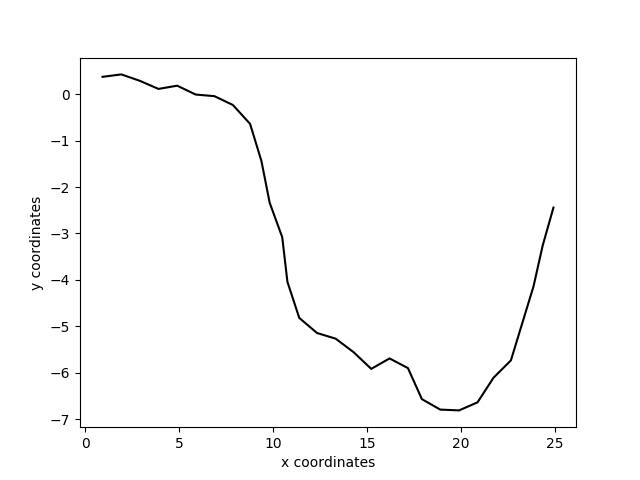
\includegraphics[scale=0.75]{images/relative_example_path.png}
\caption{Relatív random példa útvonal}
\label{fig:relative_path}
\end{figure}

\newpage

\subsection{Python program abszolút elfordulásos esetre}

Itt a generálás módja jóval egyszerűbb, ténylegesen csak egy random szám, amit nem ad hozzá az előző értékhez. Ez esetben az eredmény kevésbé reális, szinte minden útvonalban lesznek olyan szakaszok, ahol jelentős különbség van az előző és az aktuális szög között, így nagyobb törés figyelhető meg a vonalon. A program kimenete a \ref{fig:absolute_path} ábrán látható, valamint ami változott, az a generálási függvény és így a kódrészlet a következő képpen módosult:\\

\begin{python}
def generate_random_angles_absolute(number_of_turns):
    random_angles = []
    for i in range(number_of_turns):
        angle = random.randint(-35, 35)
        random_angles.append(angle)
    return random_angles
    
def calc_path(pos_x, pos_y, steering_angles):
    path = []
    for deg in steering_angles:
        pos_x = pos_x + math.cos(math.radians(deg))
        pos_y = pos_y + math.sin(math.radians(deg))
        path.append((pos_x, pos_y))
    return path
    
rand_angles_absolute = generate_random_angles_absolute(30)

random_absolute_path = calc_path(0, 0, rand_angles_absolute)

x_random_absolute = list(zip(*random_absolute_path))[0]
y_random_absolute = list(zip(*random_absolute_path))[1]

plt.plot(x_random_absolute, y_random_absolute, 'blue')
plt.xlabel("x coordinates")
plt.ylabel("y coordinates")
plt.savefig('absolute_example_path.png')
plt.show()
\end{python}

\begin{figure}[h!]
\centering
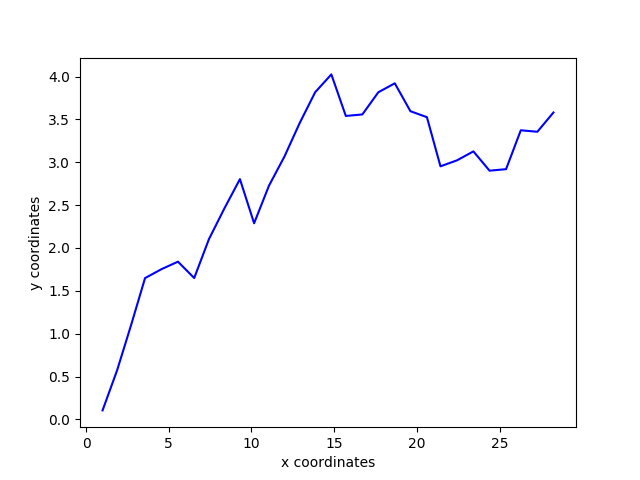
\includegraphics[scale=0.75]{images/absolute_example_path.png}
\caption{Abszolút random példa útvonal}
\label{fig:absolute_path}
\end{figure}

\newpage

\subsection{Ütközés detektálás véletlen útvonalak esetén}
Véletlen útvonalak esetén figyelmbe kell vennünk az esetleges akadályokat. Így a generált utak közül csak az lesz megfelelő, ami ezekbe nem ütközik bele. Tároljuk el ezeket mi magunk a programban, így létrehozva a környezetet. Paraméterek: obstacle(x1, y1, szélesség, magasság). Hozzáadjuk egy listához, hogy később azon végigiterálva meg tudjuk állapítani, hogy melyik obstacle objektumnál történt ütközés.

\begin{python}
obstacle1 = (2, 2, 6, 3)
obstacle2 = (8, 8, 6, 4)
obstacle3 = (15, 2, 4, 2)
obstacle4 = (8, -3, 4, 2)
obstacle5 = (23, -2, 4, 2)

obstacle_list = [obstacle1, obstacle2, obstacle3, obstacle4, obstacle5]
\end{python}

Az előző $ obstacle\_list $ listát végignézve ellenőrizzük, hogy az adott pont az akadály paraméterein belül esik-e. Ha igen, egy hamis változót igazra állítunk, valamint hozzáadjuk az adott pontot egy listához. Itt nem csak az $ x $ és $ y $ koordinátákat adom hozzá, hanem egy $ index $-et is, ami eltárolja, hogy melyik akadály objektumba ütközött az útvonal. Ha hamis, akkor a $ collided $ értéke is hamis marad. Visszatérünk két értékkel:

- volt-e ütközés

- az akadályba ütközött pontok listája

\begin{python}
def is_in_wall(x, y):
    collided = False
    collisions = []
    for index, obstacle in enumerate(obstacle_list):
        if obstacle[0] <= x <= (obstacle[0] + obstacle[2])\
                and obstacle[1] <= y <= (obstacle[1] + obstacle[3]):
            collisions.append((index, x, y))
            collided = True
    return collided, collisions
\end{python}

A már bemutatott $calc\_path$ függvényt kicsit átalakítva végig tudjuk nézni, hogy az útvonalon volt-e ütközés. Itt a for ciklus belsejében az adott pozíciót behelyettesítjük a függvény paraméterlistájába, és az első visszatérési értéket megadva feltételnek, ha az igaz, akkor hozzáadjuk az akadályba ütközött pontokat egy másik listához, amit a második visszatérési érték ad meg. Az útvonal minden eleme ugyanúgy bekerül a $ path $ listába. Majd szintén két értékkel térünk vissza:

- az útvonallal

- az akadályba ütközött pontokkal

\begin{python}
def calc_path(pos_x, pos_y, steering_angles):
    path = []
    collisions = []
    for deg in steering_angles:
        pos_x = pos_x + math.cos(math.radians(deg))
        pos_y = pos_y + math.sin(math.radians(deg))
        if is_in_wall(pos_x, pos_y)[0]:
            collisions.append(is_in_wall(pos_x, pos_y)[1])
        path.append((pos_x, pos_y))
    return path, collisions
\end{python}

Ezt a függvényt az akadályba ütközött pontok normalizálására hívom meg. Rekurzívan eltávolítja a listából a többi listát (bármennyi lehet egymásba ágyazva), így a későbbiekben egyszerűbben hivatkozhatunk a lista tuple típusú elemeire\\
($objektum\_index, x, y$). Az útvonal számító metódust meghívva, a második visszatérési értéke adja meg az ütközött pontokat.

\begin{python}
collision_list = []

def remove_nesting(nested_list):
    for i in nested_list:
        if type(i) == list:
            remove_nesting(i)
        else:
            collision_list.append(i)
            
random_relative_path_collisions = calc_path(0, 0, rand_angles_rel)[1]            
remove_nesting(random_relative_path_collisions)
\end{python}

A listába szervezett akdályokat szemléltetés képpen rajzoljuk ki a területre a \\
$ matplotlib.patches.Rectangle $ funkciót használva. Majd a $ plot() $ függvénnyel az útvonalat kirajzolni, ha pedig volt ütközés, azt legendként jelenítem meg.\\\\
Ismét bemutatnék két példa útvonalat, amelyet a hivatkozott kódrészletek segítségével generáltam ezúttal akadályokkal. Néhány futtatás után kaptunk két hasonló útvonalat, az $ y $ végpontnál talán kissé több az eltérés. Ezt minél több próbálkozással (futtatással) lehetne optimalizálni. \\\\
A \ref{fig:example_nocollision} ábrán az az útvonal látható, ahol nem volt ütközés. A \ref{fig:example_collision} ábrán pedig két objektumba is ütközött. Azokat az adatokat látjuk a legendben, ahol történt az ütközés. Az első elem, hogy melyik objektumba, a másik kettő pedig, hogy mely pontokban ütközött $ (x, y) $.

\begin{python}
plt.figure()
rectangle1 = plt.Rectangle((2, 2), 6, 3, fc='blue', ec='red')
plt.gca().add_patch(rectangle1)
rectangle2 = plt.Rectangle((8, 8), 6, 4, fc='blue', ec='red')
plt.gca().add_patch(rectangle2)
rectangle3 = plt.Rectangle((15, 2), 4, 2, fc='blue', ec='red')
plt.gca().add_patch(rectangle3)
rectangle4 = plt.Rectangle((8, -3), 4, 2, fc='blue', ec='red')
plt.gca().add_patch(rectangle4)
rectangle5 = plt.Rectangle((23, -2), 4, 2, fc='blue', ec='red')
plt.gca().add_patch(rectangle5)

plt.plot(x_random_relative, y_random_relative, 'black')
plt.xlabel("x coordinates")
plt.ylabel("y coordinates")
plt.legend(collision_list, loc='upper left', bbox_to_anchor=(0, 1.17),
handletextpad=-0.1, handlelength=0)
plt.savefig('example_nocollision.png')
plt.show()
\end{python}


\begin{figure}[h!]
\centering
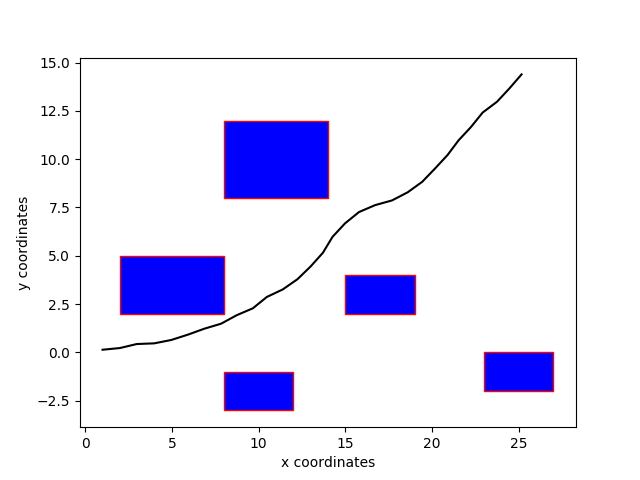
\includegraphics[scale=0.75]{images/example_nocollision.png}
\caption{Példa útvonal ütközés nélkül}
\label{fig:example_nocollision}
\end{figure}



\begin{figure}[h!]
\centering
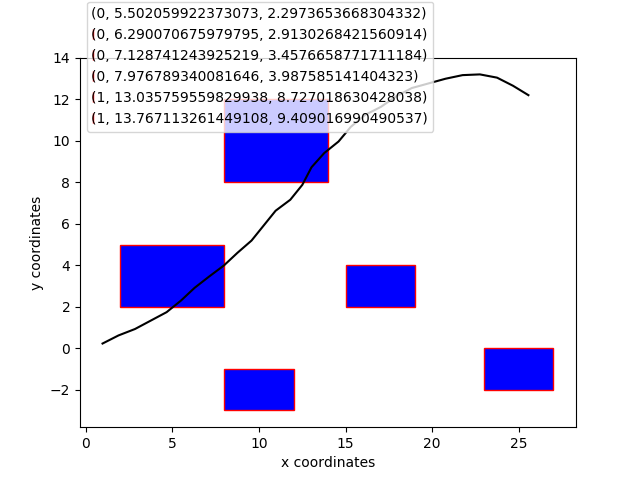
\includegraphics[scale=0.75]{images/example_collision.png}
\caption{Példa útvonal ütközéssel}
\label{fig:example_collision}
\end{figure}

\newpage

\subsection{Végpontok eloszlása, valószínűségi grafikonok}

Ebben az alpontban megvizsgáljuk, hogy különböző paraméterek esetén melyik pozícióba hány alkalommal, illetve milyen valószínűséggel juthatunk el. Legyen az alapértelmezett érték 10 000 mintaszám, tehát ennyi útvonalat fognak a függvények meghatározni. Kigyűjtöm a végpontok $ x $ és $ y $ koordinátáit 2 külön listába, ez alapján ábrázolható az értékek eloszlása.\\\\
Alap esetben legyen az elfordulások száma 30, kanyarodási szög -35$^{\circ}$, +35$^{\circ}$ közötti, generálás módszere relatív, a kezdőpozíció az origó (0, 0).\\\\
Ekkor a \ref{fig:no_obstacles_histogram2d} ábrán a (30, 0) körüli pozíciók a leggyakrabbak, de ugyanúgy gyakori eset például a (-11/+10, 28), melyek 70-70 gyakorisággal fordulnak elő.\\\\
A \ref{fig:obstacles_histogram2d} ábrán csak azokat a végpontokat látjuk, amikor egyáltalán nem volt ütközés. Ez minden esetben, 10 000 generálásnál 7000-7300 közötti rossz útvonalat számol, tehát átlagosan 2850 jó eredményből készül egy ilyen diagram. Az akadályok a \ref{fig:example_collision} vagy a \ref{fig:example_nocollision} ábrákon látható pozíciókban helyezkednek el ebben az esetben. Azt láthatjuk, hogy a leggyakoribb értékek a (12, -24/-26) pontokban lehetnek, szám szerint nagyjából 25-ször fordulnak elő. Tehát az y tengelyt tekintve inkább negatív irányba vinne minket a módszer, persze a pozitív értékeknél is léteznek útvonalak, de már csak 8-10 vagy kevesebb gyakorisággal. A világoskék színnel jelölt négyzetek is átlagban 10-szer, viszonylag gyakran fordulnak elő.



\begin{figure}[h!]
\centering
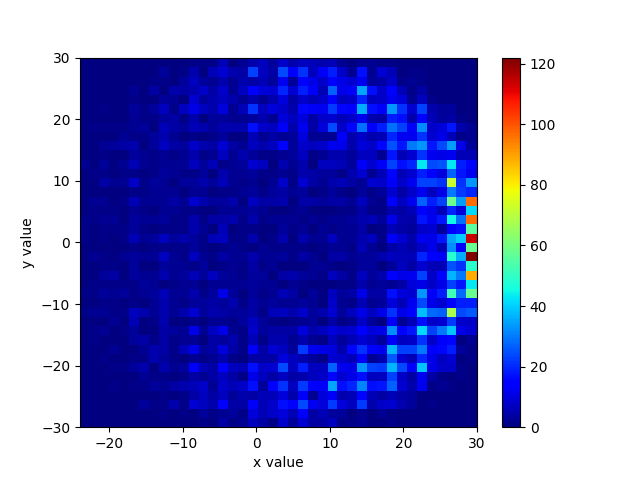
\includegraphics[scale=0.75]{images/no_obstacles_histogram2d.png}
\caption{Elérhető végpontok, ha nincs akadály a pályán}
\label{fig:no_obstacles_histogram2d}
\end{figure}

\begin{figure}[h!]
\centering
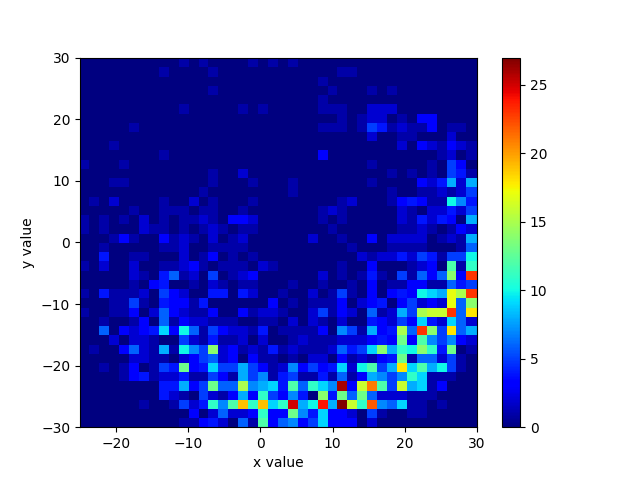
\includegraphics[scale=0.75]{images/obstacles_histogram2d.png}
\caption{Elérhető végpontok, ha vannak akadályok a pályán}
\label{fig:obstacles_histogram2d}
\end{figure}

\newpage

\subsection{Véletlen keresés eredményessége}
Ezen megoldás során inkább a relatív elfordulásos esetet vehetjük életszerűbbnek. Segítségével olyan értékeket kapunk, amelyek a kerék elfordulását határozzák meg az adott lépésben, majd így számolódik a pálya. Mivel ezek random számok, ezért nem lehet szabályozni a végeredményt. A paraméterek megfelelő beállításával kaphatunk az elvárthoz közeli eredményt, ha elegendően sok kimenetet generálunk. Ez viszont még csak egy függvényközelítési probléma, nem tekinthető optimális algoritmusnak a véletlenszerűség miatt. Ugyanakkor a jármű méreteit és irányát sem veszi figyelembe a lépések során.

\Section{Az A* algoritmus megoldása}

Következő lépésben egy olyan megoldást szeretnék bemutatni, amely segítségével bármely pontból eljuthatunk a cél pozícióba, a lehető legkisebb költséggel (jelen esetben a legrövidebb útvonalon).
Az A* algoritmust implementálva az útvonalkereséshez megkaphatjuk az elvárt eredményt. Ez egy olyan kereső eljárás, amelynek alapja a gráfszerű keresés. Minden koordinátát csomópontnak vesz és a kezdőcsúcsból indulva egyesével fűzi hozzá a csúcsokat összekötő éleket mindaddig, míg el nem éri a terminálási feltételt. Ehhez meg kell határozni egy $ f(n) = g(n) + h(n) $ függvényt, ahol $ n $ mindig a következő csúcs az úton, $ g(n) $ a kezdőcsúcstól az n-ig tartó út költsége, és $ h(n) $ egy heurisztikus függvény, amely a két pont közötti legkisebb távolságot veszi fel értékül. Minden lépésben a legkisebb értékkel rendelkező $ f $ értéket választja.
\\

\subsection{A folyamat lépései}

\begin{enumerate}
	\item Egy nyitott listát létrehozunk, majd hozzáadjuk ehhez a kezdőpontot
	\item Ismételjük a következőket, ha a nyitott lista nem üres:
	\begin{enumerate}
		\item Keressük meg a legkisebb $ f $ költségű csomópontot a nyitott listában
		\item Adjuk hozzá a zárt listához
		\item Minden szomszédos csomópontnál:
			\begin{enumerate}
				\item Ha nem járható, vagy ha a zárt listában van, akkor hagyjuk figyelmen kívül, egyébként a következőket csináljuk:
					\begin{enumerate}
						\item Ha nincs a nyitott listában, akkor adjuk hozzá és jelöljük ki a jelenlegi pontot a szülőjének, majd tároljuk el az $ f $, $ g $ és $ h $ költségeit az adott csomópontnak.
						\item Ha már a nyitott listában van, nézzük meg, hogy ez az útvonal jobb-e a $ g $ értéket vizsgálva. Ha ennek az értéke kisebb, akkor ez egy jobb útvonal az előzőnél és meg kell változtatnunk az előző pont szülőjét a jelenlegire és újra kell számítani az $ f $ és $ g $ értékeket.  
					\end{enumerate}
			\end{enumerate}
	\end{enumerate}
	\item Akkor állhatunk meg, ha a cél a zárt listához adódik, így megkaptuk a végső koordinátát, vagy ha nem találta meg valamilyen oknál fogva a célt. 
	\item Végig kell menni céltól a kezdőpontig a pontokon és így kaphatjuk meg az útvonalat
\end{enumerate}

\subsection{A környezet kialakítása}

A célom az volt, hogy egy olyan környezetben tudjam megvalósítani a keresést, amely "végtelen", tehát nincs megadva keret, hogy milyen távolságokba juthatunk el maximum, valamint hogy manuálisan lehessen megadni az akadályok pozícióit és méreteit, ezzel a tesztelést is könnyítve. Ezen kívül maga a környezet lényegében egy Descartes-féle koordináta-rendszer, amelyben a síkban egy $ P $ pont helyzete jól behatárolható $ x $ és $ y $ rendezett számpár alapján. A megjelenítés itt is szintén a matplotlib könyvtár plot() funkciójával fog majd történni.

Létre lehet hozni egy osztályt, amelyet inicializálunk az akadályokkal, ezzel kialakítva a környezetet. Ezeket egy listában tároljuk és ha szeretnénk még hozzáadni akadályokat ugyan úgy az append() funkcióval tehetjük meg. A listának tartalmaznia kell minden koordinátát, ami akadály (tehát a téglalapok keretein belül esőket is). Erre pedig egy másik függvényt hívunk meg, amely for ciklusok segítségével végigiterálva kigyűjt minden pontot az akadályokról. 

\begin{python}
import matplotlib.pyplot as plt
import numpy as np
import math


class AStarPathFinder(object):
    def __init__(self):
        self.obstacles = []
        self.obstacles.append(self.store_obstacle(2, 2, 6, 3))
        self.obstacles.append(self.store_obstacle(8, 8, 6, 4))
        self.obstacles.append(self.store_obstacle(15, 2, 4, 2))
        self.obstacles.append(self.store_obstacle(8, -3, 4, 2))
        self.obstacles.append(self.store_obstacle(23, -2, 4, 2))
        
 	def store_obstacle(self, x1, y1, width, height):
        obstacles = []
        for i in range(x1, (x1 + width + 1)):
            for j in range(y1, (y1 + height + 1)):
                obstacles.append((i, j))
        return obstacles
\end{python}

\subsection{A távolság meghatározása}

A kereső algoritmus alapja, hogy valamilyen módszerrel meg tudjuk határozni a kezdőpont és a végpont közötti távolságot. Ezzel visszakapjuk alapvetően a legrövidebb utat a két pont között. Különböző feltételeket definiálhatunk a mozgással kapcsolatban, így megemlítenék három féle ilyen távolság számítást, amik hatékonyságát a program implementálása során teszteltem.
\begin{itemize}
	\item Manhattan távolság\\
	Egyszerűbb esetekben érdemes alkalmazni, mikor a mozgás csak 4 irányba történhet az adott pontból. \\
	Képlete: 
	\begin{python}
	abs(start[0] - goal[0]) + abs(start[1] - goal[1])
	\end{python}
	\item Diagonális távolság\\
	Akkor érdemes használni, mikor 8 irányban tudunk elmozdulni az adott pontból. Jelen esetben ez is használható lenne, de az elvárt eredményhez ez sem teljesen optimális.\\
	Képlete:
	\begin{python}
	abs(start[0] - goal[0]) + abs(start[1] - goal[1])
	\end{python}
	\item Euklideszi távolság\\
	Ezt a fajta távolság becslést fogom használni, mivel minden irányban el lehet mozdulni és egy reális útvonalat kaphatunk végeredményként.\\
	Képlete a következő függvény visszatérési értéke:
\end{itemize}
\begin{python}
    def calculate_distance(self, start, goal):
        return math.sqrt(((start[0]) - goal[0]) ** 2 +
                         ((start[1]) - goal[1]) ** 2)
\end{python}

A képletek alapján ábrázolt távolságokat a  \ref{fig:distances} képen szemléltetem.

\begin{figure}[h!]
\centering
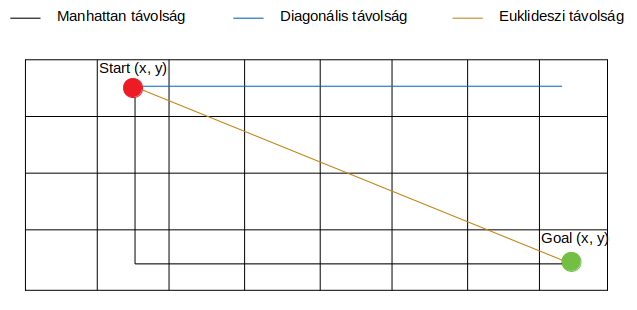
\includegraphics[scale=0.65]{images/distances.png}
\caption{Lehetséges távolságok ábrája a képletek alapján}
\label{fig:distances}
\end{figure}

\subsection{A szomszédos koordináták definiálása}

A megoldás másik elengedhetetlen funkciója, a szomszédos koordináták meghatározása, azok a pontok, amikből az adott lépésben választhatunk. Ez lehetne egyszerűen 4 irány (észak, dél, kelet, nyugat), de esetünkben nem egy labirintus-szerű térképet kell bejárni, hanem egy olyan környezetet, ahol egyedül a lehelyezett akadályokat kell kikerülni, a többi rész pedig szabadon járható. Mivel az algoritmus koordinátánként fogja a lehetőségeket vizsgálni, így az elmozdulás a pontból 8 irányban lehetséges. A \ref{fig:neighbours} ábrán jól látható, hogy az adott koordinátához képest a szomszédokat hogyan kell majd meghatározni a programban.

\begin{figure}[h!]
\centering
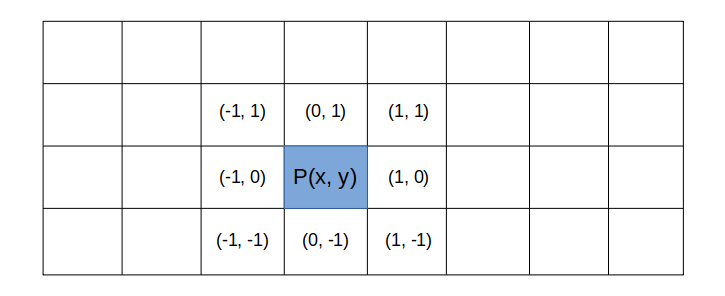
\includegraphics[scale=0.60]{images/neighbours.png}
\caption{Szomszédos koordináták a következő lépés megválasztásához}
\label{fig:neighbours}
\end{figure}

\newpage

Ehhez létre tudunk hozni egy függvényt, ami az aktuális pozíciót megkapja paraméterként. Egy listában eltárolva ezeket a szomszédos pontokat, hozzáadjuk őket egy másik listához, ami az aktuális pozíciót plusz a lehetséges szomszédokat fogja tartalmazni. 

\begin{python}
	def get_neighbours(self, position):
        neighbour = []

        for dx, dy in [(1, 0), (-1, 0), (0, 1), (0, -1),
                       (1, 1), (-1, 1), (1, -1), (-1, -1)]:
            x2 = position[0] + dx
            y2 = position[1] + dy
            neighbour.append((x2, y2))
        return neighbour 
\end{python}

\subsection{A költség meghatározása}

Szükség van egy olyan függvényre is, amely meghatározza a következő pozíció költségét. Ez egyszerűen megoldható, ha minden lépésnek 1 értékű a költsége, viszont ha ez akadályba ütközik, akkor sokkal több. Így biztosan elkerülhető, hogy az algoritmus olyan utat válasszon, ahol akadálynak ütközött.
\begin{python}
    def calc_cost(self, current, next):
        for obstacle in self.obstacles:
            if next in obstacle:
                return 100
        return 1
\end{python}

\subsection{Inputellenőrzés}
Ez a $ check\_points $ metódus csupán azt a célt szolgálja, hogy ellenőrzi a futtatáskor a felhasználó által megadott bemeneti paramétereket (jelen esetben a kezdő- és célpozíció), nem ütköznek-e akadályba. Ha igen, futásidejű hibát dob a program és a többi műveletet nem hajtja végre, ezzel elkerülve a fölösleges erőforrás használatot.
\begin{python}
	def check_points(self, start, end):
        for obstacle in self.obstacles:
            for obs in obstacle:
                if start == obs:
                    raise RuntimeError('Start coordinate is inside 
                    an obstacle!')
                elif end == obs:
                    raise RuntimeError('End coordinate is inside
                    an obstacle!')
\end{python}

\subsection{Implementáció}

Az elején ellenőrizzük, hogy helyesek-e a kezdő és végpont inputok, továbbá deklaráljuk és inicializáljuk a változókat.
\begin{python}
def a_star_search(start, end, map):

    map.check_points(start, end)

    g = {}  
    f = {}  

    g[start] = 0
    f[start] = map.heuristic(start, end)

    closed_nodes = set()
    opened_nodes = {start}
    came_from = {}
\end{python}

\bigskip

Egy while ciklusba kerülnek az ezután következő utasítások. Meg kell választani azt a koordinátát, amelyik a legkisebb $ f $ értékkel rendelkezik a nyitott listában lévőek közül, majd eltárolni jelenlegi pontnak. 
\begin{python}
	while len(opened_nodes) > 0:
        current = None
        current_f_score = None
        for pos in opened_nodes:
            if current is None or f[pos] < current_f_score:
                current_f_score = f[pos]
                current = pos

\end{python}

\bigskip

Ha elértük a végét, végig kell menni az eddig bejárt pontokon visszafelé, hogy megkapjuk a koordináták listáját. Ezeket egyesével hozzáfűzni a $ path $ listához, majd ha ez készen van, a lista elemeit az ellenkező sorrendben kell venni, hogy ne a végéről kezdődjön. Itt kapjuk meg az egész függvény visszatérési értékeit ami az útvonal, és ennek a költsége.
\begin{python}
	if current == end:
            path = [current]
            while current in came_from:
                current = came_from[current]
                path.append(current)
            path.reverse()
            return path, f[end]
\end{python}

\bigskip

A nyitott és zárt lista kezelésére folyamatos eltávolítások és hozzáadások szükségesek:

\begin{python}
	opened_nodes.remove(current)
        closed_nodes.add(current)
\end{python}

\bigskip

A következőkben az algoritmus fő változóinak értékeit fogjuk frissíteni, a szomszédos koordinátákat vizsgálva. Először megnézzük, hogy az adott szomszédos pont már a zárt listában van-e. Ha igen, akkor tovább lépünk, mivel az már fel lett dolgozva. Ha nem, akkor kiszámoltatjuk a költségét és megjelöljük, mint lehetséges következő lépést.\\

Szükséges még megvizsgálni azt is, hogy ha nincs a nyitott listában az adott csomópont. Ilyenkor hozzáadjuk és ha ennek több a költsége, mint az előbb megjelölt lehetséges pontnak, akkor tovább lépünk.\\

Mivel ez olyan ciklusban van, ami az összes szomszédot megvizsgálja, így a végén a legkisebb költségű pontot el lehet tárolni és frissítjük a $ g $, $ h $ és $ f $ változókat.\\

Ha idő előtt kilép a ciklusokból, hibával tér vissza.

\begin{python}
	for neighbour in map.get_neighbours(current):
            if neighbour in closed_nodes:
                continue
            candidate_g = g[current] + map.calc_cost(current, neighbour)

            if neighbour not in opened_nodes:
                opened_nodes.add(neighbour)
            elif candidate_g >= g[neighbour]:
                continue

            came_from[neighbour] = current
            g[neighbour] = candidate_g
            h = map.heuristic(neighbour, end)
            f[neighbour] = g[neighbour] + h

    raise RuntimeError("A* failed to find a solution")
\end{python}

\bigskip

A main függvényben meghívjuk a szükséges metódusokat és kirajzoljuk az eredményt, valamint az akadályokat is szemléltetjük. A képen piros ponttal jelöljük a kezdőpontot, zöld ponttal pedig a végpontot. Az eredményt a \ref{fig:a_star} ábrán láthatjuk.

\begin{python}
if __name__ == "__main__":
    map = AStarPathFinder()

    start = (0, 0)
    goal = (20, 3)

    path, cost = a_star_search(start, goal, map)
    x_coords = list(zip(*path))[0]
    y_coords = list(zip(*path))[1]
    
    plt.figure()
    rectangle1 = plt.Rectangle((2, 2), 6, 3, fc='blue', ec='red')
    plt.gca().add_patch(rectangle1)
    rectangle2 = plt.Rectangle((8, 8), 6, 4, fc='blue', ec='red')
    plt.gca().add_patch(rectangle2)
    rectangle3 = plt.Rectangle((15, 2), 4, 2, fc='blue', ec='red')
    plt.gca().add_patch(rectangle3)
    rectangle4 = plt.Rectangle((8, -3), 4, 2, fc='blue', ec='red')
    plt.gca().add_patch(rectangle4)
    rectangle5 = plt.Rectangle((23, -2), 4, 2, fc='blue', ec='red')
    plt.gca().add_patch(rectangle5)
    
    plt.plot(x_coords, y_coords, 'black')

    plt.plot(start[0], start[1], 'ro')
    plt.plot(goal[0], goal[1], 'go')
    plt.show()
\end{python}


\begin{figure}[h!]
\centering
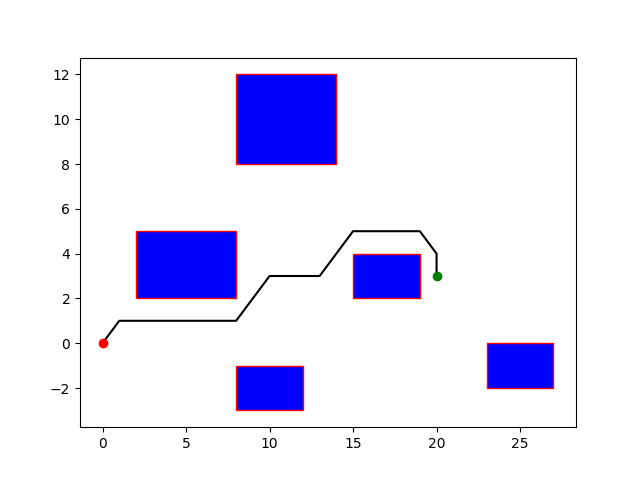
\includegraphics[scale=0.75]{images/a_star.png}
\caption{A* keresés eredménye}
\label{fig:a_star}
\end{figure}

\newpage

\subsection{A* keresés eredményessége}
Ez az algoritmus már útvonal tervezés szempontjából optimálisnak tekinthető. Jóval hatékonyabb a random keresésen alapuló módszernél olyan szempontból, hogy mi határozhatjuk meg a célpozíciót, valamint a fölösleges kanyarodásokat javarészt elkerüli. Az algoritmus a legrövidebb utat adja meg, mindig azt a pontot választja következőnek, amely a legközelebb esik a célhoz (ha az egy járható koordináta). Így ez a megoldás is tehet fölösleges irányváltoztatásokat, mert nem látja az akadályt jóval előre, csak mikor már közel van hozzá. A lehelyezett akadályok elkerülését lényegében ez az implementáció hatékonyan elvégzi, tehát biztos, hogy bármilyen bemenetre jó eredményt fogunk kapni. Másrészt azért is egy hatékony eljárás, mert emlékszik minden olyan pontra, amit már megvizsgált, és ennek függvényében tudja kiválasztani azt, ami a leghamarabb juttatná el a járművet a célba. Az irányt és a jármű méreteit itt sem vesszük figyelembe, így ez is csak egy közelítése az elérni kívánt eredménynek.

\Section{Jármű mozgásának szimulálása}

Az előző két pontban a matematikai számítások alapján készítettem egy szimulációt, ami egy parkolóban ábrázolja a téglatest alakú járművet és be lehet állítani, hogy milyen pozícióból hová jusson el. Szemléltetés képpen készítettem néhány .gif fájlt, amelyek különböző bemenetekre adnak eredményt és szemléltetik a jármű mozgását a fent leírt definíciók alkalmazásával.
\\\\
Lássuk a kódot, kezdve a szükséges importokkal és értéket adunk a konstans változóknak, amik az irányításban és a sebesség megválasztásában játszanak szerepet. Emellett a parkoló kirajzolását végző osztályt példányosítjuk.
\\\\

\begin{python}
import matplotlib.pyplot as plt
import numpy as np
from math import cos, sin, sqrt, atan2, pi
from python.program.navigator import parking_lot

k_distance = 2
k_alpha = 6
k_beta = -2
dt = 0.01

draw = parking_lot.ParkingLot()
\end{python}

\bigskip

Definiáljunk négy tömböt, melynek első két paraméterével lehet a jármű méreteit állítani, a harmadik pedig mindig 1, hogy az aktuális pozíciót adja vissza (mátrix szorzásnál vehető majd észre). Ez a négy sarkát jelenti a járműnek és az eltolások amiket megadunk, az adott tengely középpontjához mérve értendőek. Az alapértelmezett beállítás 0 radián, ekkor az autó jobbra néz, tehát az $ x $ tengely irányába. A \ref{fig:vehicle_points} ábra szemléltetné ezt a méretezést.

\begin{figure}[h!]
\centering
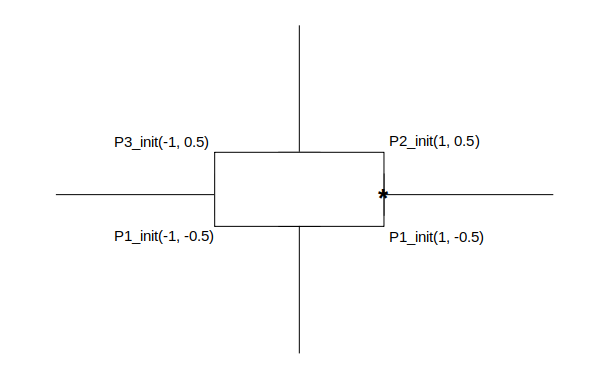
\includegraphics[scale=0.70]{images/vehicle_points.png}
\caption{A jármű négy pontja a programban}
\label{fig:vehicle_points}
\end{figure}

A programban:
\begin{python}
p1_init = np.array([1, -0.5, 1])
p2_init = np.array([1, 0.5, 1])
p3_init = np.array([-1, 0.5, 1])
p4_init = np.array([-1, -0.5, 1])
\end{python}

A rotációs mátrix egy külön függvény lesz, mely mindig az aktuális pozícióra állítja be a járművet.
\begin{python}
def rotation_matrix(x, y, heading_angle):
    return np.array([
        [cos(heading_angle), -sin(heading_angle), x],
        [sin(heading_angle), cos(heading_angle), y],
        [0, 0, 1]
    ])
\end{python}

\bigskip

A következő függvény fogja kirajzolni a járművet és az útvonalat. A pontokat megkapjuk, ha a mátrixokat a numpy.matmul() függvényével összeszorozzuk, valamint a pozíció is mindig az aktuális $ x $ és $ y $ lesz. Következő lépésben a plot() függvény segítségével összekötjük a pontokat egy vonallal, így lesz látható végig a jármű. Valamint még egy csillagot helyeztem az első részére, hogy tudjuk merre van a jármű eleje. Itt rajzoljuk ki a parkolót is, valamint kék szaggatott vonallal az útvonalat, amit egy másik függvény számol. A .gif animációhoz a képeket pedig a savefig() függvénnyel mentem le, mindig az adott lépésszámot kapja a kép neve, hogy ne íródjanak felül és legyen egy sorrend a mozgókép készítéshez.

\begin{python}
def plot_vehicle(x, y, heading_angle, x_path, y_path, steps):
    """
    Plotting the vehicle and it's path using the rotation matrix
    for visualizing.
    Plotting the parking lot as well.
    :param x: actual x position of the vehicle
    :param y: actual y position of the vehicle
    :param heading_angle: heading angle
    :param x_path: x trajectory
    :param y_path: y trajectory
    :param steps: number of steps in the motion, using for generating
    images with numbered names
    :return: none
    """
    r = rotation_matrix(x, y, heading_angle)

    p1 = np.matmul(r, p1_init)
    p2 = np.matmul(r, p2_init)
    p3 = np.matmul(r, p3_init)
    p4 = np.matmul(r, p4_init)

    plt.plot([(p1[0] + p2[0]) / 2], p1[1], 'k*')

    plt.plot([p1[0], p2[0]], [p1[1], p2[1]], 'k-')
    plt.plot([p2[0], p3[0]], [p2[1], p3[1]], 'k-')
    plt.plot([p3[0], p4[0]], [p3[1], p4[1]], 'k-')
    plt.plot([p4[0], p1[0]], [p4[1], p1[1]], 'k-')

    draw.plot_parking_lot()

    plt.plot(x_path, y_path, 'b--')
    plt.savefig('pictures/'f'fig-0{steps}.png')

\end{python}

\bigskip

A következő metódus fogja a jármű mozgatását, irányba állítását végezni a háttérben. Megadja magát az útvonalat, amit be kell járni. A szükséges változók értéket kapnak. A $ distance $ azért szerepel kétszer, mert az folyamatosan csökkenni fog, ahogy haladunk a cél felé, viszont szükség lesz a kezdőértékére is, hogy hatékonyabban tudjuk kontrollálni a sebességet ezáltal. Természetesen, ahogy az A* algoritmusnál, úgy itt is az Euklideszi távolsággal való számítás fog optimális eredményt adni.

\begin{python}
def moving_vehicle(x_start, y_start, start_heading_angle, x_goal,
 y_goal, goal_heading_angle):
    """
    Calculates the trajectory and calls vehicle plotting
    function to visualize it
    :param x_start: x start coordinate of vehicle
    :param y_start: y start coordinate of vehicle
    :param start_heading_angle: vehicle's heading angle at the start
    :param x_goal: x goal coordinate of vehicle
    :param y_goal: y goal coordinate of vehicle
    :param goal_heading_angle: vehicle's target heading angle
    at the goal position
    :return: none
    """
    x = x_start
    y = y_start
    heading_angle = start_heading_angle

    x_diff = x_goal - x
    y_diff = y_goal - y
    distance_init = sqrt(x_diff**2 + y_diff**2)
    distance = sqrt(x_diff**2 + y_diff**2)

    x_path = []
    y_path = []
\end{python}

\bigskip

A következőkben a távolság újraszámolódik, ugyanis ez minden lépésnél változni fog. A ciklus addig tart, amíg a céltól való távolság el nem ér egy nagyon kicsi értéket, jelen esetben a 0.01-et. Ezen kívül itt hozom létre azokat a szögeket, amik a \ref{fig:moving_vehicle} ábrán láthatóak. Tehát $ alpha $ az a szög, ami a jármű jelenlegi pozícióját mutató vektor és a cél felé mutató vektor által bezárt szög. Ugyanakkor a $ beta $ szög a célba érkezéshez megadott szög és a jelenlegi irány közötti szög lenne. Ezen felül a sebességet $ v $ változóként definiálom a távolsággal arányosan, valamint egy $ steering $ változót, ami végzi majd a jármű forgatását, tehát a kanyarodási szög, ami a \ref{fig:moving_vehicle} ábrán $ \gamma $ jelzéssel szerepel.

\begin{python}
while distance > 0.01:
        x_diff = x_goal - x
        y_diff = y_goal - y

        distance = sqrt(x_diff**2 + y_diff**2)
        alpha = atan2(y_diff, x_diff) - heading_angle
        beta = goal_heading_angle - heading_angle - alpha

        v = k_distance*distance
        steering = k_alpha*alpha + k_beta*beta
\end{python}

\bigskip

A sebesség kontrollálása következik. Színvonalasabb az animáció, ha a sebességet az első néhány méteren csökkentjük, vagyis utána fog növekedni a távolság függvényében. Ezzel a lassabb elindulást tehetjük láthatóvá, majd a gyorsítást. A célhoz közel pedig szintén lelassul, ez is a távolságtól függ. Másrészt beállítjuk, hogy tolasson a jármű, ha az $ alpha $ szög nagyobb mint $ \dfrac{\pi}{2} $ vagy kisebb, mint $ -\dfrac{\pi}{2} $ ( $ \alpha $ > 90$^{\circ}$ vagy $ \alpha $ < - 90$^{\circ}$ ). Ezzel a parkolóból hátrafelé kiállást valósíthatjuk meg. A tolatás sebessége egy állandó érték, ezzel megakadályozva, hogy túl gyorsan tolasson ki a távolságbecslés miatt.

\begin{python}
        if distance > distance_init - 1:
            v = v/3
        elif distance > distance_init - 2:
            v = v/2

        if alpha > pi/3 or alpha < -pi/3:
            v = -9
\end{python}

\bigskip

A $ \delta $ szöget itt a $ heading\_angle $ jelöli, ami a kanyarodás függvényében változik. Az $ x $ és $ y $ pozíciókat  hozzáadom az útvonal tárolásához létrehozott tömbökhöz, majd a kirajzoláshoz megjelenítek két nyilat, melyek a kezdő és végpozíciót reprezentálják. Ez után a már bemutatott $ plot\_vehicle $ metódus segítségével kirajzolom az útvonalat és a járművet. Ha ez a $ while $ cikluson belül történik, akkor minden lépésről képet generál, és ezekből készítettem különböző esetekre .gif animációkat. Mivel linux környezetben dolgozom, ezeket a képeket egy terminálból lefuttatott paranccsal át tudtam konvertálni: convert -delay 2 -loop 0 \$(ls -1 *.png | sort -V) animation.gif

\begin{python}
 	heading_angle = heading_angle + steering*dt

        x = x + v*cos(heading_angle)*dt
        y = y + v*sin(heading_angle)*dt
        x_path.append(x)
        y_path.append(y)

        plt.cla()
        plt.arrow(x_start, y_start, cos(start_heading_angle),
                  sin(start_heading_angle), color='r', width=0.1)
        plt.arrow(x_goal, y_goal, cos(goal_heading_angle),
                  sin(goal_heading_angle), color='g', width=0.1)
        plot_vehicle(x, y, heading_angle, x_path, y_path, len(x_path))
\end{python}

A $ main $ függvényben megadjuk a szükséges paramétereket és meghívjuk a \\ $ moving\_vehicle $ metódust. Az így kapott eredményeket a dolgozatom "animations" nevű mappájában megtalálható.

\begin{python}
if __name__ == '__main__':
    x_start = 6.5
    y_start = 8
    start_heading_angle = pi/2
    x_goal = 18.5
    y_goal = 9
    goal_heading_angle = -pi/2

    print("Start x: %.2f m\nStart y: %.2f m\nStart heading angle:
     %.2f rad\n" % (x_start, y_start, start_heading_angle))
    print("Start x: %.2f m\nGoal y: %.2f m\nGoal heading angle:
     %.2f rad\n" % (x_goal, y_goal, goal_heading_angle))
    moving_vehicle(x_start, y_start, start_heading_angle, x_goal,
     y_goal, goal_heading_angle)
\end{python}

\subsection{A jármű mozgatásának eredményessége}
Ez a megoldás jobban eltér az előzőektől. Itt az volt a szempont, hogy belekalkulálva a jármű mozgásához kapcsolódó irányváltoztatásokat és többek között a sebességet egy olyan ívelt pályán tudjunk eljutni a célba, ami az adott feltételek mellett reálisnak vehető. Tehát a sebességet, valamint a mozgás ívét is konstans értékekkel változtatva különböző eredményeket kaphatunk, mint útvonal. Ezzel a logikával könnyedén tudunk szimulációkat készíteni, mivel magát a járművet is megjeleníti, mint egy téglalap alakú objektum. Az eredmény képeket .gif formátumba átkonvertálva pedig animációkat készíthetünk. Összességében egy üres parkolóban történő navigálásra használható ez a fajta heurisztika. Amit még itt szerettem volna megvalósítani az egy nem üres parkolós környezet. Eredményesebb lenne, ha be tudná azonosítani más járművek pozícióját és észlelni, valamint elkerülni az ütközést ezen objektumokkal. 

\Chapter{Tesztelés}

% TODO: Példák kellenének, hogy egy-egy probléma megoldására hogyan használható az elkészített szoftver.


\Chapter{Összefoglalás}

Dolgozatom a négykerekű járművek alapvető navigációs problémáit elemzi, melynek alapja az útvonalkeresés. Példákon keresztül láthattunk eredményeket különböző véletlen bolyongásos kísérletekre, amelyeket összesítettem és kiértékeltem az adott paraméterek alapján. Az A* algoritmus, mint hatékony keresési eljárás segítségével megtaláltuk a legrövidebb utat két pont között egy olyan környezetben,amit a benne található akadályokkal mi magunk alakíthatunk ki és bármilyen távolságba eljuthatunk. Majd animációkkal szemléltettem a pozícionálás problémáit haladás közben. Itt szerettem volna megoldani még az ütközésdetektálás és elkerülés prolémáját, ami sajnos továbbfejlesztési lehetőségnek maradt meg. Ennél a példánál teljesen máshogy térképezi fel a bejárandó pontokat a program, mint egy gráfszerű keresés során. Így egy üres parkolót láthatunk, a terveimben pedig parkoló autók is szerepeltek, amiket jó lett volna kikerülni a mozgás közben.

Természetesen ezeken felül még további problémák is felmerülhetnek egy jármű navigálása közben. Például definiálni lehetne többféle algoritmust az útvonal meghatározására (kevesebb kanyarodással bejárható út, legkevesebb idő alatt megtehető út). Vagy olyan helyzetek kialakítása, ahol a jármű mérete is számít és emiatt újra kell terveznie az utat, vagy épp korrigálnia kell hátramenetbe kapcsolva.



\clearpage

\addcontentsline{toc}{chapter}{Irodalomjegyzék}
\bibliographystyle{plain}
\bibliography{dolgozat.bib}

\newpage

\pagestyle{empty}

\noindent \textbf{\Large A mellékelt CD tartalma}

\vskip 1cm

A dolgozathoz tartozó CD melléklet a következő elemeket tartalmazza:

\begin{itemize}
\item a dolgozatot egy \texttt{dolgozat.pdf} fájl formájában,
\item a LaTeX forráskódját a dolgozatnak a szakdolgozat jegyzékben, valamint a fejezeteket a chapters jegyzékben,
\item az elkészített programot a navigator, notebooks, positioning, random$\_$search jegyzékekben, melyek futtatásához python fordító szükséges,
\item az animations jegyzékben futási eredmények láthatóak .gif formátumban
\end{itemize}

A dolgozat és a programok a GitHub oldalán is elérhető az alábbi linken:\\
\url{https://github.com/toth135/komplex_tervezes}


\end{document}
